\documentclass[11pt]{article}
\usepackage[margin=0.9in]{geometry}
\usepackage{booktabs,longtable,array,amsmath,amssymb,hyperref,microtype,graphicx,adjustbox,pdflscape}
\usepackage[table]{xcolor}
\hypersetup{colorlinks=true,linkcolor=blue!50!black,urlcolor=blue!50!black}
\setlength{\parskip}{4pt}
\title{What produces a complexity gap:\\one economy per model and per change}
\author{Alexander Ober, with Claude}
\date{October 11, 2026; final numbers November 12; plain-language edit November 16, 2026}

\begin{document}
\maketitle


\textbf{What this report is.} Three asset-pricing models from the literature are simulated. One change is made to each at a time, the same change in all three, and every resulting economy is scored on one question: does a flexible, nonlinear portfolio method beat the best linear one out of sample? The main tables hold one economy per model per change. Everything else that was run is in Section~\ref{sec:appendix}. Every economy ran ten simulations (seeds) unless stated. The tables are built by \texttt{variants/campaign\_tables.py} from the saved results.

\textbf{Terms used throughout.}

\begin{itemize}
\item \emph{Characteristics.} The five firm variables every method sees: size, book-to-market, asset growth, profitability and momentum (plus market leverage in GS21). Methods see their ranks within each month.
\item \emph{Sharpe ratio.} A portfolio's mean excess return divided by its standard deviation. Monthly throughout; multiply by 3.5 for annual. A difference of 0.01 a month is 0.035 a year.
\item \emph{DKKM.} The nonlinear method under test (Didisheim, Kelly, Kozak and Malamud): a penalised portfolio built on thousands of random nonlinear transformations of the characteristics.
\item \emph{Classical methods.} Fama-MacBeth (FM); Fama-French factors (FF); a linear portfolio in the ranks of the characteristics, with or without the market (linear); and the estimated market line (CAPM).
\item \emph{Gap.} DKKM's out-of-sample Sharpe ratio minus the best of the four classical methods, averaged over seeds, with the t-statistic of that mean across seeds. Everything is estimated on a 360-month window. The bar for an economy to count is a gap of +0.029 a month (0.1 a year) with a clear t-statistic.
\item \emph{Best Sharpe, best linear, room.} Three numbers computed by an investor who knows the model's true conditional means and covariances. The best Sharpe is the highest attainable. The best linear is the highest a portfolio linear in the ranks attains. The room is the best nonlinear portfolio (random features, bins, quadratic terms) minus the best linear: the scope for a gap before any estimation. Room is necessary for a gap, not sufficient.
\item \emph{Type and loading.} A type is a label a firm draws at birth and keeps for life; it sets how the firm's cash flows load on the added risk factor. The loading $b_f$ is the size of that exposure.
\item \emph{Compensation.} Each type's cash-flow level is scaled so that, with the risk factor at its mean, a project's value does not depend on the type. The scaling is raised to an exponent: at 1 the correction is exact; above 1 it over-corrects, so the exposed types come out larger; below 1 it under-corrects.
\end{itemize}
\textbf{Table columns.} Model; economy (its tag and a one-line description); best Sharpe; market share (the equal-weighted market's Sharpe as a share of the best); best linear; room; room \% (room as a percentage of the best linear); interaction (the part of the best nonlinear Sharpe beyond the best linear, $\sqrt{\text{nonlinear}^2 - \text{linear}^2}$); DKKM, FM, FF, linear and CAPM (each method's out-of-sample Sharpe); gap (with its t-statistic in parentheses); DKKM extra (DKKM's Sharpe beyond the best classical method, with the sign of the gap); and + (the number of seeds with a positive gap). A dagger marks a true-moments calculation that predates the current evaluation window. GS21 methods are scored on six characteristics (the five plus leverage); a double dagger marks a GS21 economy still scored on the first five, whose method columns are not comparable.

\section{The answer}

Three models, BGN (Berk, Green and Naik 1999), GS21 (Gomes and Schmid 2021) and KP14 (Kogan and Papanikolaou 2014), are each simulated as 500 firms over 500 months. Each starts from its published calibration, and each section makes one change to it, the same change in all three.

\begin{itemize}
\item \textbf{A risk factor whose only priced event is a crash} (Section~1): no gap. Room is 3 to 12\% of the best linear Sharpe.
\item \textbf{A price of risk that rises with the square of the aggregate state} (Section~2): no gap. Room 0 to 14\%.
\item \textbf{A priced cash-flow factor that every firm bears through one of its own states} (Section~3a): no gap. Room 5 to 19\%. An exposure that only rises or only falls in one firm state is captured by the rank of the characteristic that reveals that state, however curved the exposure is.
\item \textbf{An exposure that is the product of two firm attributes}, one of them a sign the characteristics do not carry directly (Section~3b): a gap in all three. BGN +0.071, KP14 +0.181, GS21 +0.023 (at the bar).
\item \textbf{An exposure that is a U in one attribute}, the smallest and the largest firms exposed and the mid-sized not (Section~3c): a gap in all three. BGN +0.030, KP14 +0.025, GS21 +0.038 (a U in leverage: the least and the most levered firms exposed).
\item \textbf{More priced factors} (Section~4) help only when each factor's loading is itself a product of partly hidden states or the square of a characteristic. Factors that load linearly on the characteristics give nothing at any number of factors.
\end{itemize}
All ten seeds are positive in each of the six economies with a gap.

\textbf{Why these and not the others.} Every factor model is a firm's exposure times an aggregate shock. A linear portfolio in the ranks of the characteristics holds any exposure that is a sum of functions of single characteristics. A gap therefore needs an exposure with no such part: a product of two attributes that are each mean zero across firms, or a function that falls and then rises in one attribute. With one priced factor it is all or nothing. A linear portfolio with any correlation with the exposure mimics the factor, diversifies away the rest and takes the factor's whole Sharpe ratio. So the product economies need the sign hidden from the characteristics, and the U economies need the premium to rise and fall in what the characteristics reveal. Where the premium only rises or only falls in something revealed (GS21's production levels, leverage fixed by type, the KP14 U whose exposure made both exposed types the largest; Section~\ref{sec:appendix}), the linear portfolio holds it however curved the exposure.

The baselines every section is read against:

\begin{table}[htbp]\centering\footnotesize\setlength{\tabcolsep}{2pt}
\caption{Baselines. The three models as published, one type each: the floor every group is read against.}\label{tab:g0}
\begin{adjustbox}{max width=\textwidth}\begin{tabular}{l>{\raggedright\arraybackslash}p{3.6cm}rrrrrrrrrrrrrr}\hline
model & economy & \shortstack[r]{best\\Sharpe} & \shortstack[r]{market\\share} & \shortstack[r]{best\\linear} & room & \shortstack[r]{room\\\%} & \shortstack[r]{inter-\\action} & DKKM & FM & FF & linear & CAPM & gap & \shortstack[r]{DKKM\\extra} & + \\\hline
BGN & \texttt{bgnbase} -- baseline, no priced state beyond the rate & 0.301 & 54\% & 0.250 & +0.027 & 11 & 0.12 & 0.238 & 0.213 & 0.208 & 0.238 & 0.162 & -0.0001 (t -0.0) & +0.00 & 6/10 \\
GS21 & \texttt{gsbase} -- baseline & 0.293 & 95\% & 0.291 & +0.001 & 0 & 0.03 & 0.283 & 0.260 & 0.258 & 0.286 & 0.278 & -0.0028 (t -4.3) & -0.03 & 2/10 \\
KP14 & \texttt{kpbase} -- baseline, one type, no priced state & 0.229 & 35\% & 0.221 & +0.004 & 2 & 0.04 & 0.208 & 0.193 & 0.195 & 0.209 & 0.078 & -0.0010 (t -0.6) & -0.00 & 6/10 \\
\hline\end{tabular}\end{adjustbox}\end{table}


\textbf{The three models.}

\begin{itemize}
\item \emph{BGN.} A firm is a portfolio of projects. Each project costs 1, pays a lognormal cash flow $C_{jt}$ each month with its own correlation to the market shock, and dies with probability 1\% a month. One new project arrives each month and is taken if its value exceeds its cost. Two things are priced: the market shock and a mean-reverting short rate. Expected returns come from the projects' market exposure and from the growth option's exposure to the rate.
\item \emph{GS21.} Output is $Y_{it} = e^{x_t + z_{it}} k_{it}$, with aggregate productivity $x_t$ and firm productivity $z_{it}$ both mean-reverting. Cash flow to equity is $(1-\tau)(Y_{it} - (\delta + b_{it}) k_{it})$ less investment, $b_{it}$ the coupon per unit of capital. Firms invest in lumps at a random cost and may default. Aggregate productivity shocks are priced at $\gamma_x = 0.5$.
\item \emph{KP14.} Firm value is assets in place plus growth options. Project $j$ of firm $i$ pays $C_{ijt} = x_t \varepsilon_{it} u_{jt} K_j^{\alpha}$ per unit time, with $x_t$ aggregate productivity, $\varepsilon_{it}$ the firm's profitability and $u_{jt}$ the project's own, both mean-reverting around 1, and $\alpha = 0.85$. Projects arrive at a firm-specific rate and die at rate $\delta$. Two shocks are priced: aggregate productivity and embodied technology.
\item *The added risk factor $y$* (Sections~1 and 3). A mean-reverting process with unit variance and mean reversion 0.35 a year, on a grid of 21 points in BGN and 9 in GS21 and continuous in KP14; its shocks are priced at $\gamma_v = 2.5$ unless stated. A firm's cash flow is the model's own cash flow (the project cash flow $C_{jt}$ in BGN and $C_{ijt}$ in KP14, output $Y_{it}$ in GS21) times $e^{b y_t}$, with $b$ the firm's loading, and growth options are valued on the same $y$. In GS21 the coupon per unit of capital $b_i$ is drawn at birth, uniformly from 16 grid points in [0.1, 0.9], and kept for life, so cash flow to equity is $(1-\tau)(Y_{it} e^{b y_t} - (\delta + b_i) k_{it})$ less investment; $\tilde b_i = (b_i - 0.5)/0.29$ is the coupon standardised across firms. How much of the shock reaches a firm's value then depends on one state the model already has: in BGN and KP14 the share of value in assets in place rather than growth options, which book-to-market reads; in GS21 output over equity cash flow, which rises with the coupon and market leverage reads.
\item \emph{Baselines.} \texttt{bgnbase}, \texttt{gsbase} (the paper's Table I calibration) and \texttt{kpbase}: each model as published, one type, no added factor.
\end{itemize}
\section{A different distribution of shocks: a crash-only factor}

One type with one loading per model (\texttt{bvy1j}, \texttt{gvyz10j} and \texttt{vy1j}: the 3a economies with the price on ordinary shocks set to zero): 0.035 in BGN, $0.1\,\tilde z_{it}$ in GS21 ($\tilde z$ the firm's standardised productivity) and 0.07 in KP14. The factor's only priced event is a crash. Each month, with probability 1\% whatever $y_t$, $y$ jumps to $-3.5$ standard deviations (the lowest grid point; in KP14 a Poisson event at rate 0.12 a year), and the pricing rule weights that event by $e^2$, about 7\% a month under the pricing probabilities; $y$ then recovers at its ordinary speed.

\begin{table}[htbp]\centering\footnotesize\setlength{\tabcolsep}{2pt}
\caption{Group 1. A different distribution of shocks: a crash-only factor. Every firm's cash flows load on a factor y whose only priced shock is a rare crash (1\% a month to $-3.5$ sd, pricing weight $e^2$).}\label{tab:g1}
\begin{adjustbox}{max width=\textwidth}\begin{tabular}{l>{\raggedright\arraybackslash}p{3.6cm}rrrrrrrrrrrrrr}\hline
model & economy & \shortstack[r]{best\\Sharpe} & \shortstack[r]{market\\share} & \shortstack[r]{best\\linear} & room & \shortstack[r]{room\\\%} & \shortstack[r]{inter-\\action} & DKKM & FM & FF & linear & CAPM & gap & \shortstack[r]{DKKM\\extra} & + \\\hline
BGN & \texttt{bvy1j} -- crash-only factor: $e^{0.035y}$, the same crash & 0.324 & 50\% & 0.278 & +0.033 & 12 & 0.14 & 0.265 & 0.239 & 0.235 & 0.262 & 0.160 & +0.0003 (t 0.1) & +0.01 & 6/10 \\
GS21 & \texttt{gvyz10j} -- crash-only factor on $0.10\,\tilde z\,y$: y unpriced except the 1\%/month jump to $-3.5$ (weight $e^2$) & 0.386 & 82\% & 0.374 & +0.011 & 3 & 0.09 & 0.358 & 0.340 & 0.333 & 0.362 & 0.316 & -0.0046 (t -3.5) & -0.05 & 1/10 \\
KP14 & \texttt{vy1j} -- crash-only factor: $e^{0.07y}$, y unpriced except a 1\%/month jump to $-3.5$ (weight $e^2$) & 0.336 & 21\% & 0.277 & +0.012 & 4 & 0.08 & 0.259 & 0.241 & 0.249 & 0.265 & 0.066 & -0.0057 (t -2.3) & -0.04 & 2/10 \\
\hline\end{tabular}\end{adjustbox}\end{table}


\textbf{Verdict: no gap.}

\begin{itemize}
\item A crash changes the distribution of a shock that every firm bears in the same proportion. The cross-section of premia it creates is a sort on the one firm state that scales the exposure, and the linear portfolio takes nearly all of it.
\item Room is 12\% of the best linear in BGN, 3\% in GS21 and 4\% in KP14. Gaps +0.000, $-$0.005, $-$0.006.
\item Adding the same crash to the product economies instead (Section~\ref{sec:appendix}) leaves room and gap where they were in BGN and GS21 and halves KP14's.
\end{itemize}
\section{A different price of risk: quadratic in the model's own state}

The price of each model's own aggregate risk is multiplied by $1 + 0.25 s^2$, capped at 3, with $s$ a standardised aggregate state:

\begin{itemize}
\item \texttt{gq25} (GS21): $s$ is productivity $x$; the cap is 1.5.
\item \texttt{kpq} (KP14): the model's own states are random walks, so $s$ is an unpriced mean-reverting state (mean reversion 0.35, unit variance) that no firm is exposed to.
\item \texttt{bq25} (BGN): $s$ is the short rate, with the multiplier binned to seven equally likely rate levels (1.00, 1.03, 1.17 and 1.68 from the middle outward) so that project values keep a closed form; the cash flow at date $k$ is priced at the rate level one period before it pays.
\end{itemize}
The multiplier never falls below 1 because KP14's growth-option discount turns negative once the price of productivity risk drops below about 0.82 of its value.

\begin{table}[htbp]\centering\footnotesize\setlength{\tabcolsep}{2pt}
\caption{Group 2. A quadratic price of the model's own risk. The price of the baseline's aggregate risk becomes $1 + 0.25 s^2$ times its value, capped at 3, $s$ a standardized aggregate state.}\label{tab:g2}
\begin{adjustbox}{max width=\textwidth}\begin{tabular}{l>{\raggedright\arraybackslash}p{3.6cm}rrrrrrrrrrrrrr}\hline
model & economy & \shortstack[r]{best\\Sharpe} & \shortstack[r]{market\\share} & \shortstack[r]{best\\linear} & room & \shortstack[r]{room\\\%} & \shortstack[r]{inter-\\action} & DKKM & FM & FF & linear & CAPM & gap & \shortstack[r]{DKKM\\extra} & + \\\hline
BGN & \texttt{bq25} -- $\sigma_z \times \min(1 + 0.25\,s^2, 3)$, s the standardized rate, 7 bins & 0.411 & 36\% & 0.346 & +0.049 & 15 & 0.18 & 0.339 & 0.303 & 0.293 & 0.335 & 0.149 & +0.0034 (t 0.7) & +0.00 & 4/10 \\
GS21 & \texttt{gq25} -- $\gamma_x \times \min(1 + 0.25\,\tilde x^2, 3)$ & 0.345 & 95\% & 0.343 & +0.002 & 0 & 0.03 & 0.334 & 0.316 & 0.309 & 0.337 & 0.326 & -0.0036 (t -5.5) & -0.05 & 0/10 \\
KP14 & \texttt{kpq} -- $\gamma_x \times \min(1 + 0.25\,y^2, 3)$, y unpriced & 0.260 & 53\% & 0.251 & +0.003 & 1 & 0.04 & 0.240 & 0.226 & 0.225 & 0.242 & 0.137 & -0.0021 (t -1.5) & -0.02 & 4/10 \\
\hline\end{tabular}\end{adjustbox}\end{table}


\textbf{Verdict: no gap.}

\begin{itemize}
\item A price of risk that moves with the aggregate state rotates the premium across states and leaves it linear in the ranks within each state.
\item Room is under 1\% of the best linear in GS21 and KP14, and 14\% in BGN, where the rate is itself priced, so a price that rises with its distance from the mean rotates the premium with it. Gaps +0.003, $-$0.004, $-$0.002.
\item The regime-switching prices tried earlier (Section~\ref{sec:appendix}) do the same. BGN's fast regime gave the group's one small positive number (+0.008), which a linear portfolio in the ranks times the state takes.
\end{itemize}
\section{Different exposures to aggregate risk}

Every economy in this section is the baseline plus the priced factor $y$ of the front matter, with the loading set by a type.

\begin{itemize}
\item \textbf{Types.} Each firm draws a type $f$ at birth, independently of everything else, with equal shares across the types listed in each setup. The type fixes the firm's loading $b_f$ and its cash-flow level for life. The cash flow carries only $e^{b_f y_t}$; the within-firm state does the rest.
\item \textbf{The three designs.} 3a: one type, the control. 3b: types with loadings of both signs, mean zero across firms. 3c: the loading is a U in the type's position on a grid of scales, zero in the middle and positive at both ends.
\item \textbf{Compensation.} Where types differ, type $f$'s cash-flow level is multiplied by $\theta_f = (V_0/V_f)^{\omega}$, with $V_f$ the value at $y = 0$ of a unit project of type $f$. At $\omega = 1$ value at $y = 0$ does not depend on the type. $V_f$ falls in $b_f$ (under the pricing probabilities $y$ is expected to be negative), so at $\omega > 1$ size rises with $b_f$ and at $\omega < 1$ it falls. The exponent sets how visible the type is through size; 3b reports the gap across exponents.
\end{itemize}
\subsection{Exposure that a single characteristic captures}

One type, so exposure differs across firms only through the within-firm state: the assets-in-place share in BGN and KP14, the coupon in GS21.

\begin{table}[htbp]\centering\footnotesize\setlength{\tabcolsep}{2pt}
\caption{Group 3a. Exposure captured by a single characteristic. A priced state $y$ with one type and one loading on the whole cash flow: a firm's exposure varies only through one firm state (the share of value in live projects in BGN, the coupon fixed at birth in GS21, the growth-option share in KP14).}\label{tab:g3a}
\begin{adjustbox}{max width=\textwidth}\begin{tabular}{l>{\raggedright\arraybackslash}p{3.6cm}rrrrrrrrrrrrrr}\hline
model & economy & \shortstack[r]{best\\Sharpe} & \shortstack[r]{market\\share} & \shortstack[r]{best\\linear} & room & \shortstack[r]{room\\\%} & \shortstack[r]{inter-\\action} & DKKM & FM & FF & linear & CAPM & gap & \shortstack[r]{DKKM\\extra} & + \\\hline
BGN & \texttt{bvy1ch} -- one type, project cash flows $\times e^{0.035y}$ & 0.336 & 54\% & 0.297 & +0.029 & 10 & 0.13 & 0.283 & 0.252 & 0.255 & 0.281 & 0.181 & +0.0017 (t 0.8) & +0.02 & 7/10 \\
GS21 & \texttt{gvylf10} -- uniform output exposure 0.1 $y$, coupon drawn at birth from [0.1, 0.9]: leverage amplifies it (the 3a control) & 0.771 & 91\% & 0.768 & +0.002 & 0 & 0.06 & 0.752 & 0.726 & 0.733 & 0.760 & 0.703 & -0.0072 (t -5.8) & -0.10 & 0/10 \\
KP14 & \texttt{vy1} -- one type, cash flows $\times e^{0.07y}$ & 0.466 & 12\% & 0.369 & +0.019 & 5 & 0.12 & 0.355 & 0.335 & 0.340 & 0.360 & 0.047 & -0.0050 (t -2.9) & -0.05 & 1/10 \\
\hline\end{tabular}\end{adjustbox}\end{table}


\textbf{Verdict: no gap.}

\begin{itemize}
\item An exposure that only rises or only falls in one firm state, however curved, is captured by the rank of the characteristic that reveals it.
\item Room is 10\% of the best linear in BGN, 19\% in GS21 and 5\% in KP14. The gap is zero or negative in all three.
\item The same holds for every other single-characteristic economy in Section~\ref{sec:appendix}, including ones with far more room. Room is necessary, not sufficient.
\item All three estimators track the truth (Figure~\ref{fig:w3a}).
\end{itemize}
\begin{figure}[htbp]\centering
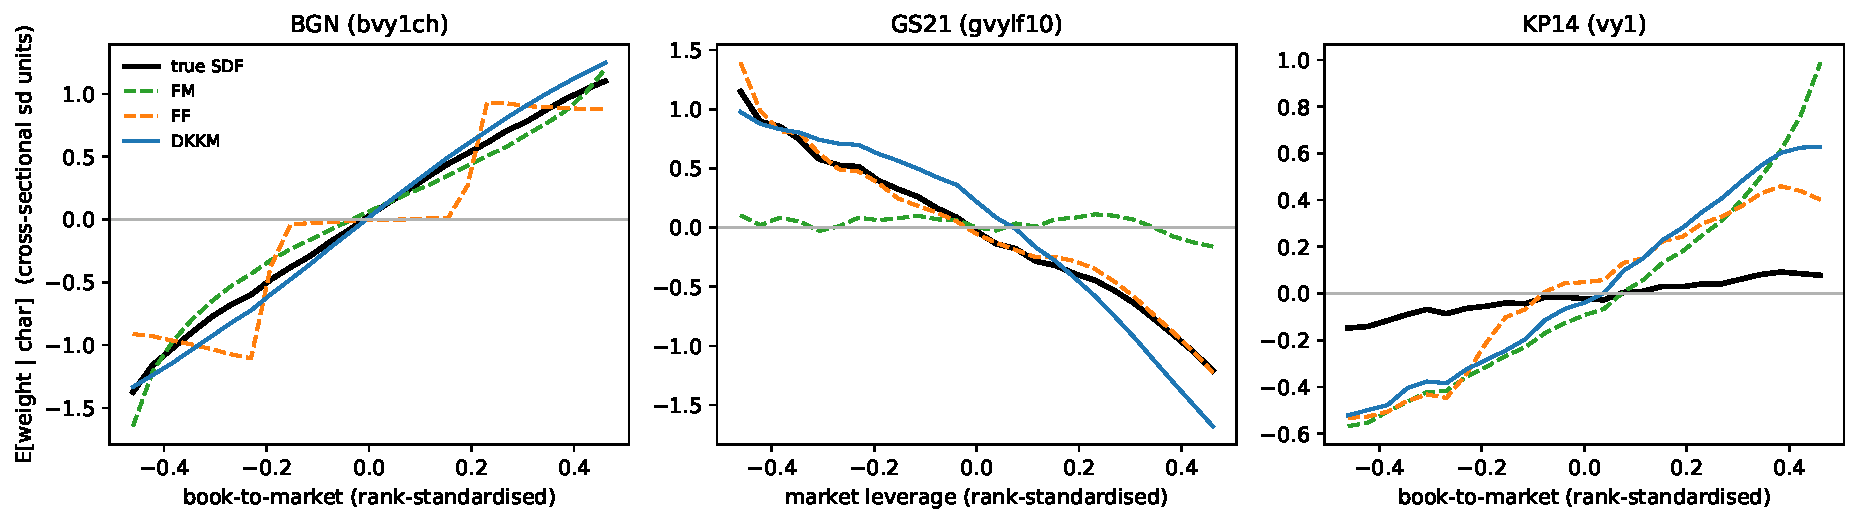
\includegraphics[width=\textwidth]{mlp_figures/sec3/fig_3a.pdf}
\caption{Portfolio weights along the 3a state: book-to-market in BGN and KP14, market leverage in GS21. Each method's per-firm weight is fitted by a small neural network on the ranked characteristics, pooled over ten seeds and the 125 evaluation months and standardised within each month; each curve is the average fitted weight at each value of the characteristic on the axis. The truth is the weight of the investor who knows the true moments; DKKM is shown at its best penalty. The true weight moves steadily along the state in BGN and GS21, and FF and DKKM sit on it in both, FM in BGN only; in KP14 the true weight is flat in book-to-market and the three estimated ones tilt toward value anyway.}\label{fig:w3a}
\end{figure}

\begin{itemize}
\item \textbf{BGN} (\texttt{bvy1ch}). \emph{Model.} Project $j$ pays $C_{jt}\,e^{0.035\,y_t}$ each month it is alive. A firm's exposure is 0.035 times the share of its value in live projects. \emph{Result.} Best linear 0.28 to 0.33, room 10\%. DKKM 0.283 against 0.282: gap +0.002 (t 0.8, seven of ten). \emph{Reading.} Book-to-market reads the share of value in live projects, so a sort on it holds the premium.
\item \textbf{GS21} (\texttt{gvylf10}). \emph{Model.} Cash flow to equity is $(1-\tau)\big(Y_{it}\,e^{0.1\,y_t} - (\delta + b_i)\,k_{it}\big)$ less investment: one loading of 0.1 on the whole of output. Equity's exposure is $0.1\,Y_{it}$ over equity cash flow, which rises with the coupon. \emph{Result.} Best linear 0.42 to 0.95 (leverage carries a premium of its own), room 0\%. DKKM 0.752 against 0.760: gap $-$0.007 (t $-$5.8, none of ten). \emph{Reading.} Market leverage reads the coupon. With the coupon written into the exponent instead, $0.1 \tilde b_i y_t$ (\texttt{gvylqs10}, Section~\ref{sec:appendix}), the exposure is convex in the coupon, room is 11 to 29\%, and the gap is still +0.000.
\item \textbf{KP14} (\texttt{vy1}). \emph{Model.} Project $j$ of firm $i$ pays $C_{ijt}\,e^{0.07\,y_t}$ per unit time. A firm's exposure is 0.07 times a weight that falls with its growth-option share. \emph{Result.} Best linear 0.35 to 0.39, room 5\%. DKKM 0.355 against 0.360: gap $-$0.005 (t $-$2.9, one of ten). \emph{Reading.} As in BGN; the growth-option share is one number per firm that size and book-to-market read.
\end{itemize}
\subsection{Exposure as a product of two attributes}

Types of equal share with loadings $\pm b_1, \pm b_2, \pm b_3$ ($\pm b_1, \pm b_2$ in GS21), mean zero across firms. The sign of $b_f$ is an industry attribute that no characteristic carries directly; how far size reveals it is set by the compensation exponent. The one-sided versions and the other levers tried are in Section~\ref{sec:appendix}.

\begin{table}[htbp]\centering\footnotesize\setlength{\tabcolsep}{2pt}
\caption{Group 3b. Exposure as an interaction of characteristics. Types with loadings of both signs drawn at birth, compensated at exponent $\omega$, times a within-firm state the type's cash flow does not carry: the assets-in-place share in BGN and KP14 (bvychs35, six types, $\omega$ = 3.5; vyg25s, six types, $\omega$ = 1.2), the coupon fixed at birth in GS21 (gvylfs6i, four types, $\omega$ = 1.2, price 6).}\label{tab:g3b}
\begin{adjustbox}{max width=\textwidth}\begin{tabular}{l>{\raggedright\arraybackslash}p{3.6cm}rrrrrrrrrrrrrr}\hline
model & economy & \shortstack[r]{best\\Sharpe} & \shortstack[r]{market\\share} & \shortstack[r]{best\\linear} & room & \shortstack[r]{room\\\%} & \shortstack[r]{inter-\\action} & DKKM & FM & FF & linear & CAPM & gap & \shortstack[r]{DKKM\\extra} & + \\\hline
BGN & \texttt{bvychs35} -- bvychs at compensation exponent 3.5 & 0.508 & 31\% & 0.294 & +0.189 & 67 & 0.38 & 0.403 & 0.315 & 0.309 & 0.303 & 0.156 & +0.0712 (t 5.8) & +0.22 & 10/10 \\
GS21 & \texttt{gvylfs6i} -- four signed types $b_f = \pm$0.03 / 0.1 on output, coupon drawn at birth from [0.1, 0.9] amplifies the sign; compensated 1.2, price 6 (gvylfs6 without its $\pm$0.2 types) & 1.344 & 39\% & 1.160 & +0.179 & 15 & 0.67 & 1.282 & 0.954 & 1.199 & 1.259 & 0.514 & +0.0232 (t 4.1) & +0.21 & 9/10 \\
KP14 & \texttt{vyg25s} -- vyg25 with sign-switching types: six types, loadings $\pm 0.02, \pm 0.07, \pm 0.14$ & 0.575 & 11\% & 0.174 & +0.349 & 226 & 0.49 & 0.373 & 0.102 & 0.190 & 0.153 & 0.056 & +0.1810 (t 17.2) & +0.32 & 10/10 \\
\hline\end{tabular}\end{adjustbox}\end{table}


\textbf{Why a product has room.}

\begin{itemize}
\item A linear portfolio in the ranks holds any sum of functions of single characteristics. The product of a loading that is mean zero across firms and a within-firm state has no such part, so no linear portfolio is long the exposure. DKKM's random features span products, and DKKM recovers part of the difference as a gap.
\item The sign does not have to be hidden. With $\omega \neq 1$ size reveals $b_f$, and the gap grows with the exponent: BGN +0.026 at 1.2 and +0.071 at 3.5; KP14 +0.116 at 0, +0.142 at 0.6, +0.181 at 1.2, +0.185 at 1.8 (Section~\ref{sec:appendix}). The product then reads as size times book-to-market, a product of two observed characteristics that the random features span and the ranks do not.
\item What is needed is the mean-zero loading. One-sided versions, in which every type loads with the same sign, are a sort on the state's characteristic with a type-dependent slope: room 10 to 27\% and no gap (Section~\ref{sec:appendix}).
\item In the estimated weights (Figure~\ref{fig:w3b}) only DKKM's curves cross.
\end{itemize}
\begin{figure}[htbp]\centering
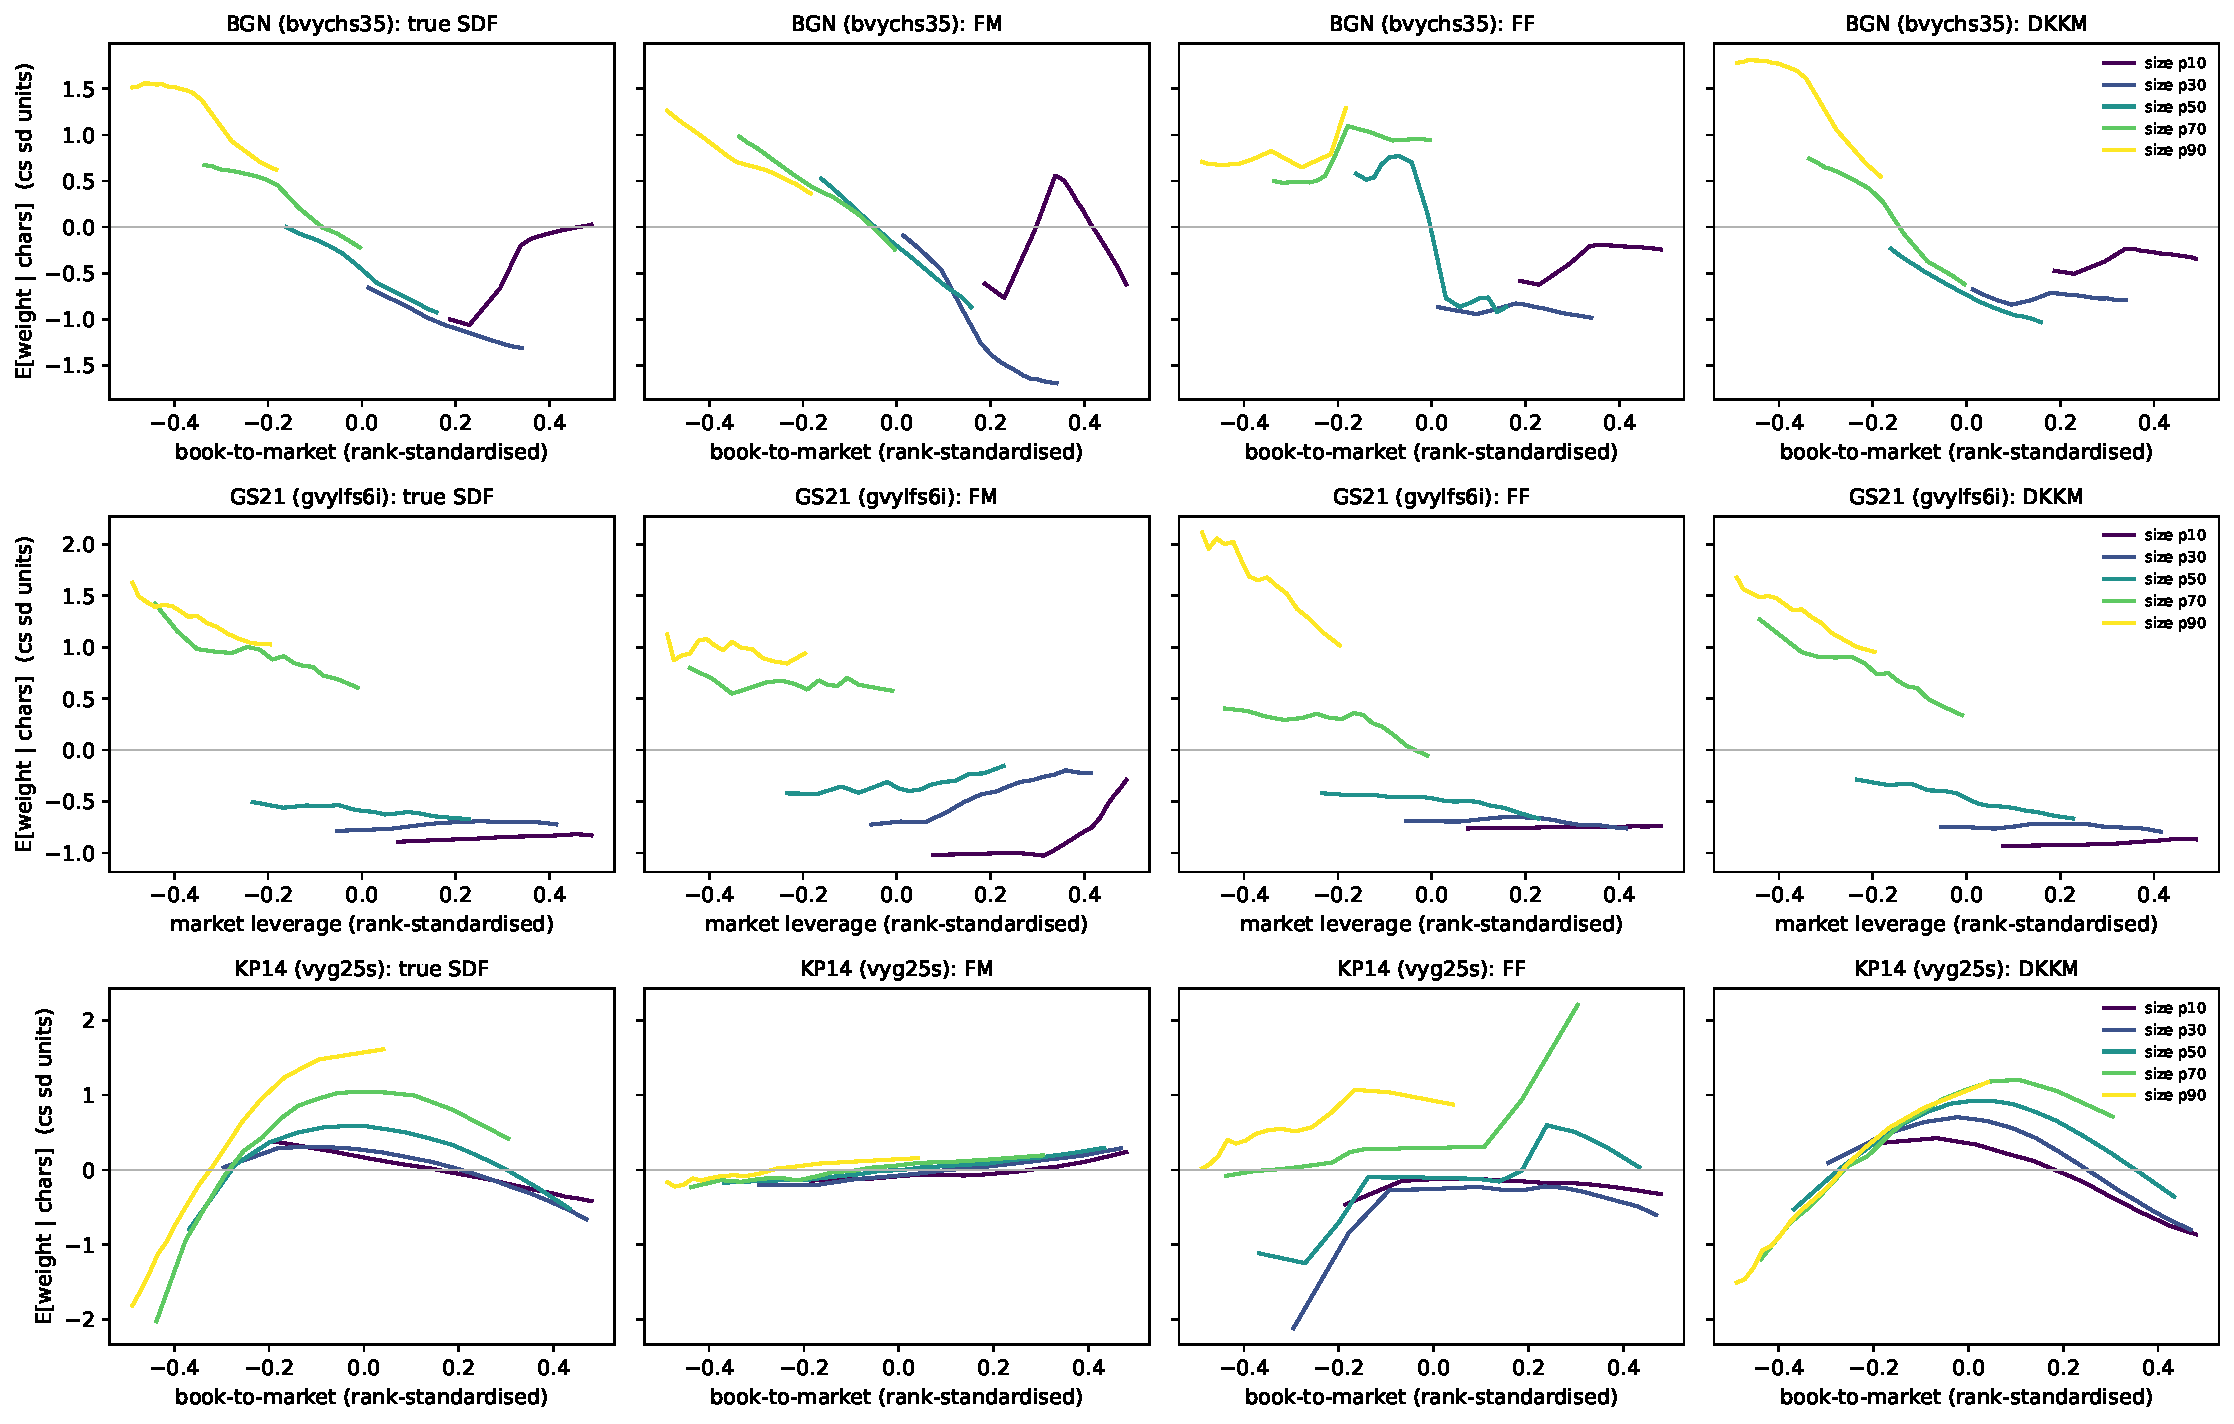
\includegraphics[width=\textwidth]{mlp_figures/sec3/fig_3b.pdf}
\caption{Weights as a function of the within-firm state at five size quantiles (size reveals the type): book-to-market in BGN and KP14, market leverage in GS21. Rows are models; columns are the true weight, FM, FF and DKKM, fitted as in the 3a figure. A product of loading and state shows as curves of different slope for small and large firms. In BGN the large firm's weight falls in book-to-market while the small firm's rises; in GS21 the large firms (the positive loadings) carry a high weight that falls in leverage while the small firms' is negative and flat; in KP14 the large firms' weight rises steeply from the low end of book-to-market and the small firms' falls at the high end. DKKM reproduces the pattern in all three; FM's curves are parallel or flat, so it holds the state's premium but not its product with the loading; FF's size-sorted steps carry most of it in GS21, a little in KP14 and none in BGN.}\label{fig:w3b}
\end{figure}

\begin{itemize}
\item \textbf{BGN} (\texttt{bvychs35}). \emph{Model.} Project $j$ of a type-$f$ firm pays $C_{jt}\,\theta_f\,e^{b_f y_t}$, with $b_f$ = $\pm$0.01, $\pm$0.035, $\pm$0.07 (six types) and $\theta_f = (V_0/V_f)^{3.5}$; price 2.5. Size ranks by type run 0.09 to 0.93 up the loadings and book-to-market ranks 0.90 down to 0.07, so both characteristics reveal $b_f$. \emph{Result.} Best linear 0.22 to 0.38, room 67\% of it. DKKM 0.403 against 0.332: gap +0.071 (t 5.8, ten of ten). Exponents 2.5 / 3.0 / 3.5 / 4.0 give +0.048 / +0.063 / +0.071 / +0.059. \emph{Reading.} Industries on opposite sides of a priced shock; within an industry the firm whose value sits in operating assets moves with it and the firm whose value sits in growth options does not. Book-to-market reads the second factor and size part of the first; no single characteristic reads the product.
\item \textbf{KP14} (\texttt{vyg25s}). \emph{Model.} Project $j$ of a type-$f$ firm pays $C_{ijt}\,\theta_f\,e^{b_f y_t}$ per unit time, with $b_f$ = $\pm$0.02, $\pm$0.07, $\pm$0.14 (six types, BGN's loadings doubled as in 3a) and $\theta_f = (V_0/V_f)^{1.2}$; price 2.5. Size ranks by type run 0.16 to 0.93 up the loadings and book-to-market ranks 0.84 down to 0.16. \emph{Result.} Best linear 0.11 to 0.28, room 97 to 382\% of it. DKKM 0.373 against 0.192 (Fama-French in eight seeds): gap +0.181 (t 17.2, ten of ten; +0.143 to +0.230). Without compensation +0.116 (t 11.1); at exponent 0.6 +0.142, at 1.8 +0.185; loadings doubled +0.245, tripled +0.218. Premium by type, in the order above: 0.56, 0.76, 0.86, 0.86, 0.84, 0.74\% a month. \emph{Reading.} As in BGN. The profitability version that held this slot (\texttt{vygelbcs}, +0.091) is in Section~\ref{sec:appendix}.
\item \textbf{GS21} (\texttt{gvylfs6i}). \emph{Model.} Cash flow to equity of a type-$f$ firm is $(1-\tau)\big(Y_{it}\,\theta_f\,e^{b_f y_t} - (\delta + b_i)\,k_{it}\big)$ less investment, with $b_f$ = $-$0.1, $-$0.03, +0.03, +0.1 (four types) and $\theta_f = (V_0/V_f)^{1.2}$; price 6. Size ranks by type run 0.02, 0.13, 0.41, 0.80 up the loadings and leverage ranks 0.78, 0.77, 0.62, 0.23 down them (seed 0); the $-$0.1 type is thin at this price (8 firms on seed 0 against 63, 131 and 130). \emph{Result.} Best linear 0.62 to 1.51 (the leverage premium, which the linear portfolio holds), room 12 to 18\%. DKKM 1.282 against 1.259 (linear in the leverage levels in every seed): gap +0.023 (t 4.1, nine of ten; $-$0.002 to +0.065). At price 2.5 room is 3 to 5\% and the gap +0.009 (t 2.1, five seeds); at price 9 room is 13 to 20\% and the gap $-$0.004. Six types with $\pm$0.2 at price 6, and the four types at exponent 3.5, did not solve (Section~\ref{sec:appendix}). Premium by type: $-$0.54, +0.01, +0.34, +0.61\% a month. \emph{Reading.} Two industries on opposite sides of the shock; within each the firm with the larger fixed payment moves more with it. Size and leverage read the industry and leverage the amplification; the product is read by neither. The gap is an eighth of KP14's because the leverage premium puts the best linear at three to five times KP14's, so the same room is a small fraction of it and DKKM recovers less. The version with the coupon in the exponent (\texttt{gvyslzg6}, +0.028) is in Section~\ref{sec:appendix}.
\end{itemize}
GS21's product without types, productivity times coupon written into production (\texttt{gvyp15}, +0.078), is the same mechanism without the industry sign. Leverage fixed by type does not work: with a few perfectly observed groups the linear portfolio prices the exposure directly (Section~\ref{sec:appendix}).

\subsection{Exposure that is a U in one attribute}

An exposure that only rises or only falls in a firm state is captured by that state's rank (3a). One that falls and then rises is not: a linear portfolio fits a line through the U and misses the curvature, which the random features see. The construction is the same in all three models.

\begin{itemize}
\item Each firm draws a type at birth, with equal shares, from five positions on a grid of scales (sixteen in GS21). $\tilde z_f$ is the type's position, standardised to mean zero and unit variance across types.
\item The loading is $b_f = c\,\tilde z_f^2$: zero for the middle type and largest at the two ends, so the firms at both extremes carry the exposure and the firms in the middle none.
\item The scale is what the characteristic reads. In BGN it is the firm scale (project cost, cash flows, book and value all scaled by the type, so only size moves). In KP14 it is the cash-flow level, a pure scale there as well: investment adjusts, and book-to-market and profitability do not move. In GS21 it is the coupon per unit of capital, which market leverage reads.
\item In BGN and KP14 the five positions give $b_f$ = 0.35, 0.09, 0, 0.09, 0.35. The exposure itself adds to value (0.6 log units of size per unit loading in BGN, 14 in KP14, where investment amplifies it), so the scales are set so that the five types occupy the five fifths of the size distribution after that effect. In GS21 the coupon is drawn from 16 points and $b_f = 0.5\,\tilde b_f^2$ runs from 0 at the middle coupon to 0.95 at the ends.
\item Compensation at exponent 1, price 2.5.
\item A loading of one sign at both ends is what the earlier hump ($-c, 0, +c, 0, -c$) and the signed U ($\tilde b^2 - 1$) did not have; those are in Section~\ref{sec:appendix}.
\end{itemize}
\begin{table}[htbp]\centering\footnotesize\setlength{\tabcolsep}{2pt}
\caption{Group 3c. Exposure non-monotone in a characteristic. One blueprint in all three: types drawn at birth with equal shares, each at a position $\tilde z_f$ on a grid of scales, with the loading $b_f = c\,\tilde z_f^2$, zero in the middle and positive at both ends, compensated at $y = 0$, price 2.5. In BGN (bvyuq2) the grid is the firm scale and in KP14 (vyuq2) the cash-flow level, five positions set so the types occupy the fifths of size, $b_f$ = 0.35, 0.09, 0, 0.09, 0.35; in GS21 (gvylqup5) it is the coupon drawn from 16 nodes in [0.1, 0.9], $b_f = 0.5\,\tilde b_f^2$ from 0 at the middle coupon to 0.95 at the ends.}\label{tab:g3c}
\begin{adjustbox}{max width=\textwidth}\begin{tabular}{l>{\raggedright\arraybackslash}p{3.6cm}rrrrrrrrrrrrrr}\hline
model & economy & \shortstack[r]{best\\Sharpe} & \shortstack[r]{market\\share} & \shortstack[r]{best\\linear} & room & \shortstack[r]{room\\\%} & \shortstack[r]{inter-\\action} & DKKM & FM & FF & linear & CAPM & gap & \shortstack[r]{DKKM\\extra} & + \\\hline
BGN & \texttt{bvyuq2} -- loading $c\tilde z^2$ on firm scales [1.0, 0.33, 0.61, 1.49, 1.99] (firm scale; solved so the types sit at the fifths of size), $b$ = 0.35, 0.09, 0, 0.09, 0.35, price 2.5 & 0.751 & 55\% & 0.522 & +0.142 & 30 & 0.40 & 0.554 & 0.471 & 0.475 & 0.524 & 0.411 & +0.0302 (t 6.1) & +0.18 & 10/10 \\
KP14 & \texttt{vyuq2} -- loading $c\tilde z^2$ on cash-flow levels [1.0, 0.38, 0.74, 0.92, 0.58] (solved so the types sit at the fifths of size), $b$ = 0.35, 0.09, 0, 0.09, 0.35, price 2.5 & 0.484 & 8\% & 0.307 & +0.103 & 34 & 0.27 & 0.318 & 0.179 & 0.264 & 0.294 & 0.022 & +0.0245 (t 9.2) & +0.12 & 10/10 \\
GS21 & \texttt{gvylqup5} -- sixteen coupon types drawn at birth from [0.1, 0.9], loading $b_f = 0.5\,\tilde b_f^2$ (zero at the middle coupon, +0.95 at the ends), unbounded, compensated at $y = 0$ & 1.272 & 84\% & 1.095 & +0.163 & 15 & 0.62 & 1.138 & 1.052 & 1.030 & 1.099 & 1.061 & +0.0376 (t 4.3) & +0.27 & 10/10 \\
\hline\end{tabular}\end{adjustbox}\end{table}


\begin{figure}[htbp]\centering
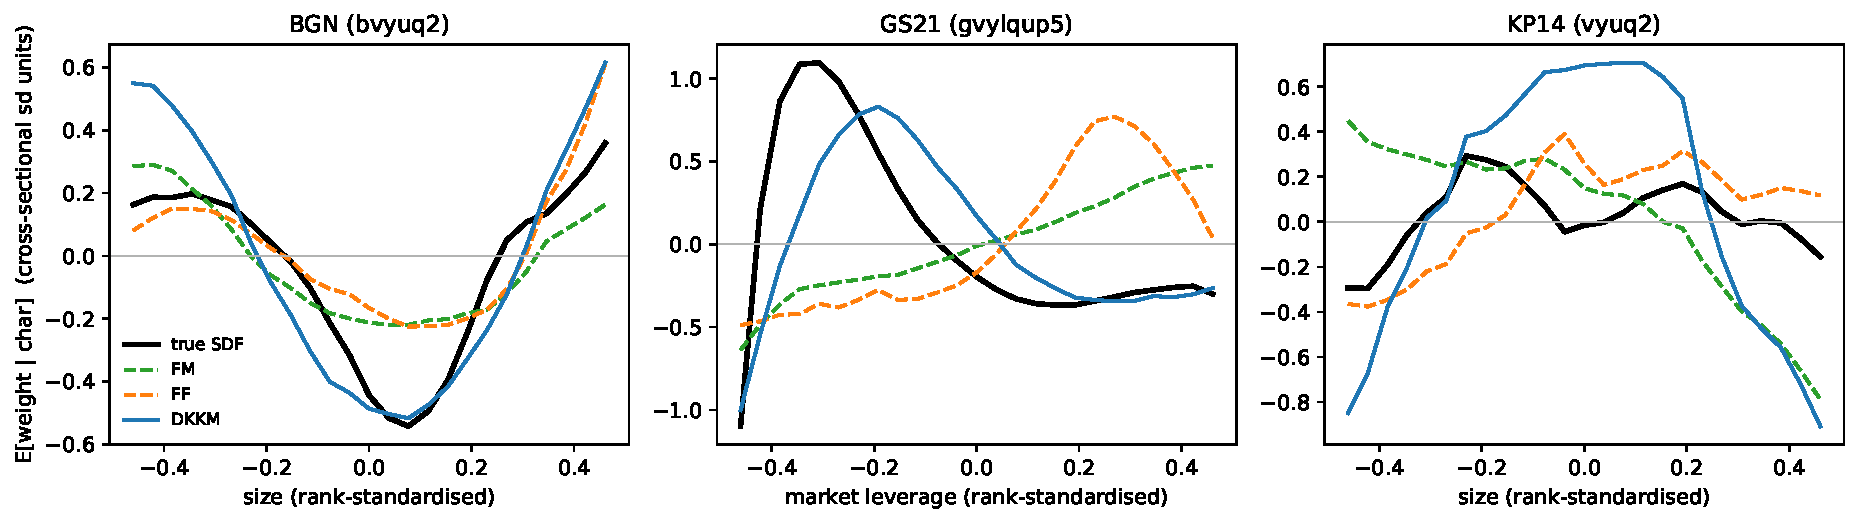
\includegraphics[width=\textwidth]{mlp_figures/sec3/fig_3c.pdf}
\caption{Weights along the attribute the U is written on: size in BGN and KP14 (five types, the exposed ones at both ends), market leverage in GS21, fitted as in the 3a figure. The true weight is a U in size in BGN, short the unexposed middle type and long both ends; in KP14 a hump with a dip at the middle, short both exposed ends; in GS21 a peak at low leverage that falls through the rest of the range. DKKM follows the shape in all three. FM fits a line through the hump in KP14 and through the leverage profile in GS21, and in BGN a shallower U through book-to-market, which the exposed types share.}\label{fig:w3c}
\end{figure}

\begin{itemize}
\item \textbf{BGN} (\texttt{bvyuq2}). \emph{Model.} A type-$f$ firm's projects cost $s_f$ and pay $s_f\,C_{jt}\,\theta_f\,e^{b_f y_t}$, with the scale $s_f$ = 0.33, 0.61, 1.0, 1.49, 1.99, $b_f = 0.35\,\tilde z_f^2$ = 0.35, 0.09, 0, 0.09, 0.35 in the same order, and $\theta_f = V_0/V_f$; price 2.5. Size rank by type 0.18, 0.30, 0.52, 0.69, 0.86: the exposed types are the smallest and the largest. \emph{Result.} Best linear 0.35 to 0.72, room 8 to 51\%. DKKM 0.554 against 0.524: gap +0.030 (t 6.1, ten of ten; +0.010 to +0.062). Premium by type, in the order of size: 4.6, 1.2, 0.6, 1.2, 4.6\% a month, a U in size. The exposed types have market betas of 1.5 against 0.65 to 0.75 and alphas of +1.0 against $-$0.4 to $-$0.8\% a month. Exposure also raises book-to-market (0.97 against 0.78 to 0.81), profitability and momentum, so the ranks of the five characteristics explain 67\% of the loading's variance across firms, book-to-market most; what they leave is the pairing of the smallest firms with the largest. The true weight by type, in standard-deviation units and in the order of size, is +0.32, +0.30, $-$1.18, +0.30, +0.30: short the unexposed middle and long every other type. DKKM's is +0.74, $-$0.05, $-$0.76, $-$0.31, +0.49 and FM's +0.55, $-$0.13, $-$0.36, $-$0.28, +0.24, a shallower U reached through book-to-market. \emph{Reading.} Small firms exposed through financing constraints, the largest through operating leverage, the mid-sized through neither. The premium is a U in size, and a portfolio linear in the size rank holds a slope through it.
\item \textbf{KP14} (\texttt{vyuq2}). \emph{Model.} Project $j$ of a type-$f$ firm pays $C_{ijt}\,\theta_f\,\ell_f\,e^{b_f y_t}$ per unit time, with the cash-flow level $\ell_f$ = 0.38, 0.74, 1.0, 0.92, 0.58 (in the order of size; the exposed types' set below the middle type's to offset the size the exposure adds), $b_f$ = 0.35, 0.09, 0, 0.09, 0.35 and $\theta_f = V_0/V_f$; price 2.5. Size rank by type 0.14, 0.29, 0.53, 0.69, 0.89. The level moves neither book-to-market nor profitability. \emph{Result.} Best linear 0.29 to 0.33, room 26 to 41\%. DKKM 0.318 against 0.294: gap +0.025 (t 9.2, ten of ten; +0.015 to +0.042). Premium by type, in the order of size: 0.17, 0.41, 0.51, 0.41, 0.18\% a month. The exposed types earn less, a hump in size: their market beta is higher (1.11 against 0.83 in seed 0) and their alpha lower ($-$0.21 against +0.23\% a month). This is KP14's pricing, not the construction. In every KP14 type economy the premium peaks near a loading of zero and falls on either side (in 3b it runs 0.56 up to 0.86 and back to 0.74 across the loadings), while in BGN the exposed types earn the most. Exposure lowers book-to-market (0.006 against 0.34), so book-to-market reveals who is exposed and size which end. The true weight by type is $-$0.28, +0.38, $-$0.24, +0.38, $-$0.26: short both exposed types and long the lightly exposed ones beside them, because exposure adds variance faster than premium; along size a hump with a dip in the middle. DKKM's is $-$0.82, +0.67, +0.62, +0.51, $-$1.05, a hump, and FM's +0.29, +0.24, +0.31, $-$0.22, $-$0.63, a line down size. \emph{Reading.} The smallest and largest firms carry the shock and the mid-sized do not. In KP14 the shock's premium is small next to the market premium, so the exposed firms, with the higher beta but the lower alpha, earn less. The exposure is a U in size and the premium a hump, and neither is a line in the size rank.
\item \textbf{GS21} (\texttt{gvylqup5}). \emph{Model.} Cash flow to equity of a type-$f$ firm is $(1-\tau)\big(Y_{it}\,\theta_f\,e^{b_f y_t} - (\delta + c_f)\,k_{it}\big)$ less investment, with $c_f$ the $f$-th of the 16 coupon points in [0.1, 0.9] (sixteen types), $\tilde b_f = (c_f - 0.5)/0.29$, $b_f = 0.5\,\tilde b_f^2$ (0 at the middle coupon, 0.95 at the ends) and $\theta_f = 1/W(b_f)$, where $W(e) = \sum_k e^{-rk}\,\mathbb{E}^Q[e^{e y_k}] / \sum_k e^{-rk}$ is the value under the pricing probabilities of the exposure stream per unit of a riskless annuity, so that value at $y = 0$ does not reveal $b_f$; price 2.5. \emph{Result.} Best linear 0.65 to 1.34 (the leverage premium), room 7 to 18\%. DKKM 1.138 against 1.100: gap +0.038 (t 4.3, ten of ten; +0.004 to +0.085). Premium across leverage quintiles, averaged over seeds: 9.7, 2.7, 1.5, 2.6, 6.6\% a month, a U in leverage, with market betas 2.3, 0.55, 0.28, 0.51, 1.33. At twice the loading (\texttt{gvylqup10}) the gap is +0.072 (t 6.1) but the least levered quintile earns 28\% a month and is twelve times the size of the next, which rules it out. The true weight across the quintiles is +0.15, +0.60, $-$0.16, $-$0.34, $-$0.25: long the second quintile most, while the least levered firms, whose premium is the largest, carry little weight because their beta (2.3) and volatility are the largest too; a peak at low leverage rather than a U. DKKM's is $-$0.35, +0.71, +0.19, $-$0.28, $-$0.27 and FM's $-$0.37, $-$0.16, $-$0.02, +0.16, +0.39, a line up leverage. \emph{Reading.} Unlevered firms are credit rationed and highly levered firms in distress; both are more sensitive to the shock than the firm of middling leverage, and the premium is a U in leverage. The signed U (\texttt{gvylqun10}, +0.027), the humps, the U in a distance-to-distress index (\texttt{gvylqzu5g4}, +0.055) and the productivity hump (\texttt{gvyzzh10}, +0.080) are in Section~\ref{sec:appendix}.
\end{itemize}
In each of the three the exposure is a U in the attribute the characteristic reads, and the ranks of the characteristics span a slope through it and not the curvature. The premium follows the exposure in BGN and GS21 and is a hump in KP14; either way it rises and falls in what the characteristics reveal.

\section{Larger factor models}

The three sections above change one feature of a structural model. This one asks whether more priced factors help, in a reduced form whose structure is fully controlled: a panel of firms with five characteristics, a market factor, and $K$ extra priced factors whose total price of risk is held fixed as $K$ grows. The only thing that varies across the rows is what the extra factors load on: a linear function of the observed characteristics, a product of two partly hidden firm states (Section~3b's design), or the square of one firm state (Section~3c's). The structural version, a second priced state in each model, is in Section~\ref{sec:appendix}.

\textbf{The reduced form.} 500 firms over 500 months after a 100-month burn-in, five seeds per cell, scored exactly as the structural economies; its true conditional moments are known in closed form. $i$ indexes firms, $t$ months, $j$ the five characteristics and $k$ the extra factors.

\begin{itemize}
\item \emph{Firm states.} Each firm carries five independent mean-reverting processes $z_{ijt}$ with persistence (0.99, 0.98, 0.90, 0.95, 0.70) and unit variance.
\item \emph{Observed characteristics.} $X_{ijt} = z_{ijt}$ in the kfh and kfo families. In the lfh family each characteristic is its state plus observation noise with standard deviation $\sigma_\nu$: 0 (rows n0) or 1, as large as the state itself (rows n1). Methods see the ranks of $X$, as everywhere in the report.
\item \emph{Returns.} $r_{i,t+1} = B_{it}\lambda + B_{it} f_{t+1} + \varepsilon_{i,t+1}$, with factor shocks of standard deviation 0.04 and firm noise 0.10, all independent; $B_{it}$ holds the firm's loadings and $\lambda$ the prices of risk.
\item \emph{The market factor.} Loading $1 + 0.3\,(\tilde{\mathrm{bm}} + \tilde{\mathrm{roe}} + \tilde{\mathrm{mom}})$ on the standardised characteristics, price 0.002 (a Sharpe of 0.05). It is linear in the characteristics, so every method holds it.
\item *The $K$ extra factors.* Price $0.024/\sqrt{K}$ each, so the total price of risk is the same at every $K$. Every extra loading is centred across firms each month, so the equal-weighted market carries none of the extra premia. The families differ only in the loading:
\begin{itemize}
\item \emph{kfh}: a function of a fixed random direction in the characteristics ($h(u) = u$ in the main table; $\tanh$ and the square in Section~\ref{sec:appendix}). Exposure is a function of what the characteristics show directly.
\item \emph{kfo} (Section~\ref{sec:appendix}): kfh with the size coordinate removed, so no extra factor loads on size.
\item \emph{lfh}: the product of two of the five states, one pair per factor (so $K \le 10$), which the characteristics reveal only up to the observation noise: Section~3b's design.
\item \emph{lsq, lsqb, lsqr}: the square of one state (size, book-to-market or profitability), $z^2 - 1$, observed exactly (n0) or with noise (n1): Section~3c's design.
\end{itemize}
\item In the kfh families the best Sharpe falls at $K = 16$ because sixteen directions over five characteristics are collinear and partly cancel; in the lfh family it stays near 0.6 at every $K$.
\end{itemize}
\begin{table}[htbp]\centering\footnotesize\setlength{\tabcolsep}{2pt}
\caption{Reduced form: priced factors loading linearly on observed characteristics, on products of two partly hidden firm states, and on the square of one firm state (size, book-to-market or profitability). Five seeds per cell, the total price of risk fixed across K (per-factor price $\propto 1/\sqrt{K}$); K = number of priced factors; the lfh rows load products of pairs of the five latent processes, observed with noise of sd 0 (n0) or 1 (n1).}\label{tab:rf}
\begin{adjustbox}{max width=\textwidth}\begin{tabular}{>{\raggedright\arraybackslash}p{4.6cm}rrrrrrrrrrrrr}\hline
configuration & \shortstack[r]{best\\Sharpe} & \shortstack[r]{market\\share} & \shortstack[r]{best\\linear} & room & \shortstack[r]{room\\\%} & \shortstack[r]{inter-\\action} & DKKM & FM & FF & linear & CAPM & gap & + \\\hline
\multicolumn{14}{l}{\textit{Linear loadings on observed characteristics}} \\
kfh\_lin\_1 -- K=1 factor on observed characteristics, linear loadings & 0.598 & 8 & 0.598 & +0.000 & 0 & 0.01 & 0.590 & 0.584 & 0.581 & 0.595 & 0.041 & -0.0067 (t -1.7) & 0/5 \\
kfh\_lin\_4 -- K=4 & 0.592 & 8 & 0.588 & +0.003 & 0 & 0.06 & 0.555 & 0.578 & 0.567 & 0.575 & 0.041 & -0.0237 (t -3.1) & 0/5 \\
kfh\_lin\_16 -- K=16 & 0.385 & 13 & 0.383 & +0.001 & 0 & 0.03 & 0.352 & 0.357 & 0.353 & 0.365 & 0.041 & -0.0128 (t -1.2) & 2/5 \\
\hline
\multicolumn{14}{l}{\textit{Interactions: products of two partly hidden firm states}} \\
lfh\_L5\_K1\_n0 -- K=1 product of latent states, no observation noise & 0.598 & 8 & 0.208 & +0.389 & 187 & 0.56 & 0.570 & 0.156 & 0.539 & 0.175 & 0.041 & +0.0311 (t 4.0) & 5/5 \\
lfh\_L5\_K2\_n0 -- K=2 & 0.598 & 8 & 0.144 & +0.453 & 314 & 0.58 & 0.564 & 0.111 & 0.520 & 0.115 & 0.041 & +0.0443 (t 6.7) & 5/5 \\
lfh\_L5\_K3\_n0 -- K=3 & 0.598 & 8 & 0.106 & +0.490 & 464 & 0.59 & 0.566 & 0.059 & 0.507 & 0.084 & 0.041 & +0.0589 (t 9.0) & 5/5 \\
lfh\_L5\_K5\_n0 -- K=5 & 0.598 & 8 & 0.092 & +0.502 & 549 & 0.59 & 0.543 & 0.048 & 0.423 & 0.064 & 0.041 & +0.1193 (t 21.6) & 5/5 \\
lfh\_L5\_K10\_n0 -- K=10 & 0.598 & 8 & 0.089 & +0.503 & 568 & 0.58 & 0.507 & 0.047 & 0.250 & 0.067 & 0.041 & +0.2572 (t 39.9) & 5/5 \\
lfh\_L5\_K1\_n1 -- K=1 product of latent states, observation noise 1.0 & 0.598 & 8 & 0.167 & +0.416 & 249 & 0.56 & 0.526 & 0.096 & 0.433 & 0.137 & 0.041 & +0.0930 (t 3.8) & 5/5 \\
lfh\_L5\_K2\_n1 -- K=2 & 0.598 & 8 & 0.111 & +0.469 & 423 & 0.57 & 0.523 & 0.072 & 0.420 & 0.082 & 0.041 & +0.1025 (t 6.8) & 5/5 \\
lfh\_L5\_K3\_n1 -- K=3 & 0.598 & 8 & 0.091 & +0.486 & 537 & 0.57 & 0.528 & 0.057 & 0.391 & 0.073 & 0.041 & +0.1371 (t 10.4) & 5/5 \\
lfh\_L5\_K5\_n1 -- K=5 & 0.598 & 8 & 0.075 & +0.496 & 664 & 0.57 & 0.496 & 0.038 & 0.309 & 0.060 & 0.041 & +0.1866 (t 26.3) & 5/5 \\
lfh\_L5\_K10\_n1 -- K=10 & 0.598 & 8 & 0.079 & +0.479 & 607 & 0.55 & 0.456 & 0.052 & 0.171 & 0.077 & 0.041 & +0.2854 (t 24.8) & 5/5 \\
\hline
\multicolumn{14}{l}{\textit{Non-monotone exposures: the square of one firm state}} \\
lsq\_a0\_n0 -- K=1, square of size, mean zero, state observed exactly & 0.598 & 8 & 0.175 & +0.422 & 242 & 0.57 & 0.557 & 0.153 & 0.565 & 0.151 & 0.041 & -0.0082 (t -1.5) & 2/5 \\
lsq\_a0\_n1 -- observation noise 1.0 & 0.598 & 8 & 0.144 & +0.436 & 302 & 0.56 & 0.508 & 0.119 & 0.540 & 0.130 & 0.041 & -0.0313 (t -2.0) & 1/5 \\
lsqb\_a0\_n0 -- K=1, square of book-to-market, mean zero, observed exactly & 0.598 & 8 & 0.199 & +0.398 & 200 & 0.56 & 0.564 & 0.142 & 0.125 & 0.173 & 0.041 & +0.3662 (t 11.0) & 5/5 \\
lsqb\_a0\_n1 -- noise 1.0 & 0.598 & 8 & 0.190 & +0.392 & 206 & 0.55 & 0.515 & 0.120 & 0.092 & 0.146 & 0.041 & +0.3403 (t 6.5) & 5/5 \\
lsqr\_a0\_n0 -- K=1, square of profitability, mean zero, observed exactly & 0.598 & 8 & 0.121 & +0.476 & 392 & 0.58 & 0.569 & 0.076 & 0.064 & 0.101 & 0.041 & +0.4462 (t 11.9) & 5/5 \\
lsqr\_a0\_n1 -- noise 1.0 & 0.598 & 8 & 0.111 & +0.471 & 425 & 0.57 & 0.532 & 0.012 & 0.049 & 0.058 & 0.041 & +0.4574 (t 17.5) & 5/5 \\
\hline\end{tabular}\end{adjustbox}\end{table}


\textbf{Findings.}

\begin{itemize}
\item Factors that load linearly on observed characteristics leave no room at any $K$ and a negative gap.
\item Factors that load on products of partly hidden states give room and a gap that grow with $K$ and with the noise that hides the states, to +0.29 at ten factors with noise. A product of two mean-zero states has no part a linear portfolio can hold, and each extra factor adds another product.
\item A square is a U. Squaring book-to-market (lsqb) gives room +0.40 and a gap of +0.37 (t 11) with the state observed exactly, and +0.34 with noise. Squaring size (lsq) gives the same room and no gap: market value is $e^{\mathrm{size}}$, so the value-weighted market inside the Fama-French set holds size squared mechanically, and FF reaches 0.57 of a best Sharpe of 0.60. Squaring profitability (lsqr) gives the largest of the three: room +0.48, about four times the best linear, and a gap of +0.446 (t 11.9) with the state observed exactly and +0.457 (t 17.5) with noise, five of five each. Shifting the mean of the squared state, $(z + m)^2 - 1$, adds a linear part and sends the room to near zero at $m$ of 1 or more (Section~\ref{sec:appendix}), as the shifted products do for the interaction.
\end{itemize}
\textbf{The structural version} (\texttt{vym3s}, \texttt{vym6s}; rows in the Section~\ref{sec:appendix} table): one set of mean-zero types spread over $K$ priced states. $K$ independent mean-reverting states, each priced $2.5/\sqrt{K}$; 24 mean-zero types of equal share with loading vectors of size 0.07 or 0.14 at cosines $\pm$1, $\pm$0.84, $\pm$0.68, $\pm$0.52, $\pm$0.36, $\pm$0.20 to the price vector; compensation exponent 1.2. Both are \texttt{vyg25s} with its types spread over $K$ states.

\begin{itemize}
\item The best linear is unchanged (0.191 and 0.192 against 0.174), but the best Sharpe falls from 0.575 to 0.503 and 0.507: a type whose loading is misaligned with the price vector carries the full risk of its size and earns only the cosine of the premium.
\item Room is 0.224 and 0.225 (110\% of the best linear against 201\%), and DKKM takes the same 71\% of the best nonlinear Sharpe as in \texttt{vyg25s}: 0.296 against FM's 0.134 and the linear portfolio's 0.196, a gap of +0.100 (t 21) and +0.099 (t 15), ten of ten at either $K$, the second largest of the campaign and half of \texttt{vyg25s}'s.
\item $K = 3$ and $K = 6$ agree to the third digit. In the structural models, unlike the reduced form, more priced states do not multiply interactions, because every state acts through the one growth-option channel. The one-signed construction at $K = 6$ (\texttt{vym6}) reproduces \texttt{vym3} (room 19\%, gap +0.000): $K$ itself is not a lever.
\end{itemize}
\section{Additional economies}\label{sec:appendix}

Everything else that was run. The table has the main tables' columns, and the bullets describe each economy against its parent. Three groups answer side questions: the crash added to the product economies (\texttt{bvyj25}, \texttt{gvyp10j}, \texttt{vyj25}), the GS21 product family (\texttt{gvyp05} to \texttt{gvyp20}, \texttt{gvyp10x}), and the earlier single-characteristic and price-of-risk designs that the harmonised cells replace.

\begin{landscape}\footnotesize\setlength{\tabcolsep}{2pt}
\begin{longtable}{lp{4.6cm}rrrrrrrrrrrrrr}
\caption{Additional economies, BGN. Everything else that was run, by model, each described in the appendix against its parent; the RF rows are the reduced-form families with bounded (tanh), curvature (square) and size-orthogonal curvature (kfo) loadings, the sign construction (lsh: the K=1 latent product with the factors' means shifted; lrt: a one-signed ratio), and the curvature-in-a-latent family (lsq / lsqb: the square of one partly hidden latent, size or book-to-market, with its mean shifted).}\label{tab:xa-bgn}\\\hline
model & economy & \shortstack[r]{best\\Sharpe} & \shortstack[r]{market\\share} & \shortstack[r]{best\\linear} & room & \shortstack[r]{room\\\%} & \shortstack[r]{inter-\\action} & DKKM & FM & FF & linear & CAPM & gap & \shortstack[r]{DKKM\\extra} & + \\\hline\endfirsthead
\multicolumn{16}{l}{\textit{Additional economies, BGN (continued)}}\\\hline
model & economy & \shortstack[r]{best\\Sharpe} & \shortstack[r]{market\\share} & \shortstack[r]{best\\linear} & room & \shortstack[r]{room\\\%} & \shortstack[r]{inter-\\action} & DKKM & FM & FF & linear & CAPM & gap & \shortstack[r]{DKKM\\extra} & + \\\hline\endhead
\hline\endfoot
BGN & \texttt{g0235f} -- regime price $\times$0.2 / $\times$3.5, spells 4$\times$ faster & 0.237 & 62\% & 0.163 & +0.045 & 28 & 0.13 & 0.169 & 0.141 & 0.131 & 0.161 & 0.146 & +0.0079 (t 4.8) & +0.05 & 10/10 \\
BGN & \texttt{g0235df} -- stress 2/3 of the time, 4$\times$ faster & 0.489 & 17\% & 0.432 & +0.036 & 9 & 0.18 & 0.423 & 0.392 & 0.351 & 0.428 & 0.077 & -0.0051 (t -2.2) & -0.05 & 2/10 \\
BGN & \texttt{bvy25} -- three types on y, compensated (1.2) & 0.601 & 41\% & 0.398 & +0.062 & 16 & 0.23 & 0.399 & 0.344 & 0.367 & 0.384 & 0.248 & +0.0148 (t 3.0) & +0.09 & 9/10 \\
BGN & \texttt{bvych41} -- bvych0 on a 41-point grid & 0.565 & 38\% & 0.336 & +0.052 & 15 & 0.19 & 0.328 & 0.279 & 0.291 & 0.320 & 0.215 & +0.0086 (t 2.8) & +0.06 & 8/10 \\
BGN & \texttt{bvyc0} -- the same without compensation & 0.475 & 41\% & 0.395 & +0.066 & 18 & 0.22 & 0.386 & 0.321 & 0.347 & 0.376 & 0.195 & +0.0104 (t 3.1) & +0.07 & 9/10 \\
BGN & \texttt{bvyj25} -- the chain with a priced crash (1\%/month to $-y_{\max}$, pricing weight $e^2$) & 0.536 & 38\% & 0.315 & +0.054 & 17 & 0.19 & 0.307 & 0.261 & 0.269 & 0.301 & 0.202 & +0.0066 (t 2.8) & +0.05 & 9/10 \\
BGN & \texttt{bvysg} -- signed loadings ($-0.07$ / 0 / $+0.07$) & 0.504 & 28\% & 0.361 & +0.120 & 35 & 0.31 & 0.318 & 0.305 & 0.273 & 0.324 & 0.141 & -0.0199 (t -2.0) & -0.08 & 2/10 \\
BGN & \texttt{bvy9t2} -- two priced chains, nine types (independent loadings), total price 2.5 & 0.636 & 42\% & 0.398 & +0.063 & 16 & 0.23 & 0.395 & 0.339 & 0.355 & 0.383 & 0.266 & +0.0124 (t 3.5) & +0.08 & 8/10 \\
BGN & \texttt{bvychs} -- bvych0 with sign-switching types: six types, loadings $\pm 0.01, \pm 0.035, \pm 0.07$ & 0.510 & 36\% & 0.349 & +0.069 & 20 & 0.23 & 0.360 & 0.274 & 0.277 & 0.334 & 0.183 & +0.0255 (t 4.9) & +0.12 & 9/10 \\
BGN & \texttt{bvychs4} -- bvychs at compensation exponent 0.4 & 0.612 & 29\% & 0.519 & +0.059 & 12 & 0.25 & 0.497 & 0.468 & 0.465 & 0.497 & 0.177 & -0.0035 (t -0.3) & -0.01 & 2/5 \\
BGN & \texttt{bvychs6} -- bvychs at compensation exponent 0.6 & 0.656 & 28\% & 0.578 & +0.047 & 8 & 0.23 & 0.547 & 0.493 & 0.512 & 0.545 & 0.183 & +0.0013 (t 0.3) & +0.00 & 1/3 \\
BGN & \texttt{bvychs8} -- bvychs at compensation exponent 0.8 & 0.684 & 28\% & 0.590 & +0.044 & 7 & 0.23 & 0.577 & 0.501 & 0.468 & 0.568 & 0.189 & +0.0086 (t 1.0) & +0.06 & 2/3 \\
BGN & \texttt{bvychs18} -- bvychs at compensation exponent 1.8 & 0.340 & 49\% & 0.207 & +0.055 & 27 & 0.16 & 0.218 & 0.198 & 0.178 & 0.208 & 0.167 & +0.0064 (t 1.4) & +0.03 & 6/8 \\
BGN & \texttt{bvychs25} -- bvychs at compensation exponent 2.5 & 0.449 & 36\% & 0.250 & +0.163 & 67 & 0.33 & 0.341 & 0.286 & 0.223 & 0.246 & 0.159 & +0.0482 (t 3.7) & +0.15 & 9/10 \\
BGN & \texttt{bvychs30} -- bvychs at compensation exponent 3.0 & 0.488 & 32\% & 0.277 & +0.182 & 67 & 0.36 & 0.384 & 0.318 & 0.268 & 0.279 & 0.157 & +0.0626 (t 5.6) & +0.20 & 10/10 \\
BGN & \texttt{bvychs35} -- bvychs at compensation exponent 3.5 & 0.508 & 31\% & 0.294 & +0.189 & 67 & 0.38 & 0.403 & 0.315 & 0.309 & 0.303 & 0.156 & +0.0712 (t 5.8) & +0.22 & 10/10 \\
BGN & \texttt{bvychs40} -- bvychs at compensation exponent 4.0 & 0.518 & 30\% & 0.305 & +0.189 & 65 & 0.39 & 0.413 & 0.305 & 0.334 & 0.319 & 0.155 & +0.0590 (t 4.6) & +0.20 & 10/10 \\
BGN & \texttt{bvychs45} -- bvychs at compensation exponent 4.5 & 0.525 & 29\% & 0.281 & +0.224 & 81 & 0.42 & 0.422 & 0.316 & 0.345 & 0.315 & 0.154 & +0.0638 (t 2.5) & +0.21 & 4/4 \\
BGN & \texttt{bvychsn5} -- bvychs at compensation exponent -0.5 & 0.367 & 35\% & 0.254 & +0.080 & 35 & 0.21 & 0.229 & 0.202 & 0.207 & 0.228 & 0.127 & -0.0054 (t -0.9) & -0.01 & 6/10 \\
BGN & \texttt{bvyvee} -- V-shaped loading across cash-flow levels 0.6..1.4, $b$ = +0.07, +0.00, -0.07, +0.00, +0.07 & 0.485 & 34\% & 0.352 & +0.076 & 23 & 0.24 & 0.352 & 0.305 & 0.320 & 0.344 & 0.164 & +0.0071 (t 1.3) & +0.05 & 6/8 \\
BGN & \texttt{bvyhx2} -- hump-shaped loading across cash-flow levels 0.85..1.15: $b$ = -0.14, +0.00, +0.14, +0.00, -0.14 & 0.597 & 27\% & 0.526 & +0.057 & 11 & 0.25 & 0.523 & 0.392 & 0.315 & 0.508 & 0.158 & +0.0150 (t 0.7) & +0.06 & 2/3 \\
BGN & \texttt{bvyhx3} -- hump-shaped loading across cash-flow levels 0.8..1.2: $b$ = -0.21, +0.00, +0.21, +0.00, -0.21 & 0.551 & 28\% & 0.349 & +0.155 & 44 & 0.36 & 0.375 & 0.295 & 0.280 & 0.340 & 0.153 & +0.0345 (t 3.9) & +0.14 & 10/10 \\
BGN & \texttt{bvyhx4} -- hump-shaped loading across cash-flow levels 0.8..1.2: $b$ = -0.28, +0.00, +0.28, +0.00, -0.28 & 0.642 & 25\% & 0.357 & +0.260 & 73 & 0.50 & 0.476 & 0.341 & 0.293 & 0.344 & 0.159 & +0.1186 (t 10.9) & +0.31 & 10/10 \\
BGN & \texttt{bvyhsc} -- hump-shaped loading $\pm$0.28 across a firm scales [0.6, 0.78, 1.0, 1.28, 1.65] (only size moves) & 0.522 & 31\% & 0.362 & +0.120 & 33 & 0.32 & 0.354 & 0.295 & 0.297 & 0.345 & 0.160 & +0.0093 (t 1.2) & +0.06 & 5/6 \\
BGN & \texttt{bvyhsw} -- hump-shaped loading $\pm$0.28 across a firm scales [0.4, 0.63, 1.0, 1.58, 2.5] (only size moves) & 0.529 & 30\% & 0.357 & +0.135 & 38 & 0.34 & 0.354 & 0.290 & 0.290 & 0.339 & 0.159 & +0.0146 (t 1.8) & +0.08 & 4/5 \\
BGN & \texttt{bvyus3} -- U-shaped loading in size: +0.35 on the two ends of a firm scales [1.0, 0.6, 1.65] (only size moves), three types, price 2.5 & 0.741 & 60\% & 0.538 & +0.142 & 30 & 0.40 & 0.601 & 0.468 & 0.491 & 0.542 & 0.450 & +0.0587 (t 15.0) & +0.26 & 10/10 \\
BGN & \texttt{bvyuq35} -- loading $c\tilde z^2$ on firm scales [1.0, 0.6, 0.78, 1.28, 1.65] (only size moves), $b$ = 0.35, 0.09, 0, 0.09, 0.35, price 3.5 & 0.953 & 47\% & 0.637 & +0.194 & 34 & 0.52 & 0.703 & 0.554 & 0.566 & 0.641 & 0.449 & +0.0625 (t 7.6) & +0.28 & 10/10 \\
BGN & \texttt{bvyuq2h} -- loading $c\tilde z^2$ on firm scales [1.0, 0.33, 0.61, 1.49, 1.99] (firm scale; solved so the types sit at the fifths of size), $b$ = 0.35, 0.09, 0, 0.09, 0.35, price 3.5 & 0.953 & 47\% & 0.637 & +0.201 & 35 & 0.53 & 0.701 & 0.556 & 0.567 & 0.640 & 0.449 & +0.0599 (t 7.7) & +0.28 & 10/10 \\
BGN & \texttt{bvyuq2} -- loading $c\tilde z^2$ on firm scales [1.0, 0.33, 0.61, 1.49, 1.99] (firm scale; solved so the types sit at the fifths of size), $b$ = 0.35, 0.09, 0, 0.09, 0.35, price 2.5 & 0.751 & 55\% & 0.522 & +0.142 & 30 & 0.40 & 0.554 & 0.471 & 0.475 & 0.524 & 0.411 & +0.0302 (t 6.1) & +0.18 & 10/10 \\
BGN & \texttt{bvyuq} -- loading $c\tilde z^2$ on firm scales [1.0, 0.6, 0.78, 1.28, 1.65] (only size moves), $b$ = 0.35, 0.09, 0, 0.09, 0.35, price 2.5 & 0.751 & 55\% & 0.523 & +0.137 & 29 & 0.39 & 0.553 & 0.471 & 0.478 & 0.522 & 0.411 & +0.0301 (t 5.9) & +0.18 & 10/10 \\
BGN & \texttt{bvyq2} -- two chains, the second loading quadratic in the first: $b_2 = -14\,(b_1^2 - \bar{b_1^2})$, $b_1 = \pm$0.01, $\pm$0.035, $\pm$0.07 & 0.460 & 37\% & 0.303 & +0.063 & 21 & 0.20 & 0.307 & 0.240 & 0.260 & 0.285 & 0.172 & +0.0223 (t 18.1) & +0.11 & 3/3 \\
BGN & \texttt{bvyq2x} -- two chains, the second loading quadratic in the first: $b_2 = -7\,(b_1^2 - \bar{b_1^2})$, $b_1 = \pm$0.02, $\pm$0.07, $\pm$0.14 & 0.523 & 30\% & 0.375 & +0.070 & 19 & 0.24 & 0.359 & 0.321 & 0.308 & 0.366 & 0.158 & -0.0075 (t -1.2) & -0.05 & 1/3 \\
BGN & \texttt{bvyq2k} -- two chains, the second loading quadratic in the first: $b_2 = -28\,(b_1^2 - \bar{b_1^2})$, $b_1 = \pm$0.01, $\pm$0.035, $\pm$0.07 & 0.470 & 34\% & 0.315 & +0.071 & 22 & 0.22 & 0.304 & 0.265 & 0.261 & 0.302 & 0.159 & +0.0026 (t 0.9) & +0.01 & 6/10 \\
BGN & \texttt{bvyu6r} -- U-shaped loading across cash-flow levels 0.8..1.2: $b$ = +0.42 at the ends, unexposed reference type & 0.768 & 49\% & 0.592 & +0.137 & 24 & 0.42 & 0.616 & 0.479 & 0.533 & 0.582 & 0.373 & +0.0246 (t 2.6) & +0.13 & 8/10 \\
BGN & \texttt{bvyu5r} -- U-shaped loading across cash-flow levels 0.8..1.2: $b$ = +0.35 at the ends, unexposed reference type & 0.774 & 46\% & 0.641 & +0.108 & 17 & 0.38 & 0.664 & 0.562 & 0.558 & 0.623 & 0.358 & +0.0295 (t 3.1) & +0.16 & 9/10 \\
BGN & \texttt{bvyu4} -- U-shaped loading across cash-flow levels 0.8..1.2: $b$ = +0.28, 0, 0, 0, +0.28 & 0.382 & 31\% & 0.246 & +0.111 & 54 & 0.25 & 0.241 & 0.157 & 0.181 & 0.227 & 0.118 & +0.0142 (t 1.3) & +0.06 & 7/10 \\
BGN & \texttt{bvych0} -- y as a 21-point grid, three types (control) & 0.576 & 37\% & 0.341 & +0.055 & 16 & 0.20 & 0.334 & 0.285 & 0.292 & 0.326 & 0.216 & +0.0076 (t 2.7) & +0.05 & 8/10 \\
BGN & \texttt{bvychsx2} -- bvychs with the loadings x 2: $\pm$0.02, $\pm$0.07, $\pm$0.14 & 0.496 & 32\% & 0.344 & +0.089 & 26 & 0.26 & 0.347 & 0.308 & 0.279 & 0.333 & 0.161 & +0.0072 (t 1.1) & +0.04 & 7/10 \\
BGN & \texttt{bvychsx3} -- bvychs with the loadings x 3: $\pm$0.03, $\pm$0.105, $\pm$0.21 & 0.533 & 31\% & 0.384 & +0.081 & 21 & 0.26 & 0.377 & 0.353 & 0.321 & 0.370 & 0.164 & +0.0024 (t 0.5) & +0.01 & 6/10 \\
\end{longtable}

\begin{longtable}{lp{4.6cm}rrrrrrrrrrrrrr}
\caption{Additional economies, GS21. Columns as in the other tables.}\label{tab:xa-gs21}\\\hline
model & economy & \shortstack[r]{best\\Sharpe} & \shortstack[r]{market\\share} & \shortstack[r]{best\\linear} & room & \shortstack[r]{room\\\%} & \shortstack[r]{inter-\\action} & DKKM & FM & FF & linear & CAPM & gap & \shortstack[r]{DKKM\\extra} & + \\\hline\endfirsthead
\multicolumn{16}{l}{\textit{Additional economies, GS21 (continued)}}\\\hline
model & economy & \shortstack[r]{best\\Sharpe} & \shortstack[r]{market\\share} & \shortstack[r]{best\\linear} & room & \shortstack[r]{room\\\%} & \shortstack[r]{inter-\\action} & DKKM & FM & FF & linear & CAPM & gap & \shortstack[r]{DKKM\\extra} & + \\\hline\endhead
\hline\endfoot
GS21 & \texttt{g28} -- countercyclical $\gamma(x)$, clipped & 0.314 & 95\% & 0.312 & +0.001 & 0 & 0.02 & 0.303 & 0.254 & 0.256 & 0.305 & 0.298 & -0.0024 (t -4.3) & -0.04 & 0/10 \\
GS21 & \texttt{bx7} -- two-state regime on $\gamma$, five types on x & 0.327 & 94\% & 0.317 & +0.007 & 2 & 0.07 & 0.309 & 0.282 & 0.271 & 0.311 & 0.306 & -0.0017 (t -2.8) & -0.03 & 0/10 \\
GS21 & \texttt{gx7} -- five types on productivity x & 0.485 & 98\% & 0.474 & +0.008 & 2 & 0.08 & 0.473 & 0.393 & 0.383 & 0.473 & 0.473 & +0.0003 (t 1.6) & +0.01 & 5/10 \\
GS21 & \texttt{gvy1} -- one type, output $\times e^{0.05y}$ & 0.636 & 95\% & 0.633 & +0.002 & 0 & 0.05 & 0.626 & 0.608 & 0.598 & 0.629 & 0.602 & -0.0030 (t -4.0) & -0.05 & 1/10 \\
GS21 & \texttt{gvy1j} -- crash-only factor: $e^{0.05y}$, the same crash & 0.379 & 96\% & 0.377 & +0.001 & 0 & 0.03 & 0.372 & 0.350 & 0.341 & 0.374 & 0.363 & -0.0022 (t -4.4) & -0.04 & 1/10 \\
GS21 & \texttt{gvy25} -- production-level exposure to y, three types & 0.725 & 86\% & 0.709 & +0.014 & 2 & 0.14 & 0.688 & 0.682 & 0.666 & 0.695 & 0.625 & -0.0070 (t -4.0) & -0.09 & 1/10 \\
GS21 & \texttt{gvys25} -- signed fixed-cost exposure to y & 0.619 & 69\% & 0.602 & +0.014 & 2 & 0.13 & 0.496 & 0.490 & 0.426 & 0.499 & 0.420 & -0.0032 (t -1.5) & -0.03 & 2/6 \\
GS21 & \texttt{gvyp05} -- product $\tilde z\tilde b$ at 0.05 & 0.425 & 60\% & 0.284 & +0.128 & 45 & 0.30 & 0.297 & 0.254 & 0.202 & 0.276 & 0.254 & +0.0203 (t 7.4) & +0.11 & 10/10 \\
GS21 & \texttt{gvyp075} -- product at 0.075 & 0.561 & 28\% & 0.261 & +0.287 & 111 & 0.48 & 0.433 & 0.212 & 0.187 & 0.352 & 0.149 & +0.0802 (t 9.4) & +0.25 & 10/10 \\
GS21 & \texttt{gvyp15} -- product at 0.15 & 0.744 & -25\% & 0.616 & +0.119 & 22 & 0.39 & 0.665 & 0.349 & 0.516 & 0.612 & 0.192 & +0.0528 (t 9.3) & +0.26 & 10/10 \\
GS21 & \texttt{gvyp20} -- product at 0.20 & 0.778 & -51\% & 0.729 & +0.039 & 6 & 0.23 & 0.710 & 0.452 & 0.643 & 0.715 & 0.407 & -0.0049 (t -1.1) & -0.04 & 4/10 \\
GS21 & \texttt{gvyp10x} -- product at 0.10 plus a curvature loading on x & 0.589 & 17\% & 0.365 & +0.215 & 63 & 0.45 & 0.491 & 0.196 & 0.262 & 0.448 & 0.054 & +0.0431 (t 7.6) & +0.20 & 10/10 \\
GS21 & \texttt{gvyp10j} -- the product exposure with a priced crash & 0.537 & 21\% & 0.328 & +0.197 & 62 & 0.41 & 0.442 & 0.242 & 0.246 & 0.415 & 0.072 & +0.0267 (t 3.8) & +0.14 & 10/10 \\
GS21 & \texttt{gvypk2} -- two priced chains, two product types & 0.478 & 27\% & 0.226 & +0.212 & 103 & 0.37 & 0.309 & 0.168 & 0.153 & 0.254 & 0.105 & +0.0559 (t 3.2) & +0.15 & 9/10 \\
GS21 & \texttt{gvyzl} -- productivity exposure, three fixed-coupon leverage types (diluting) & 0.865 & 50\% & 0.793 & +0.059 & 8 & 0.31 & 0.804 & 0.793 & 0.743 & 0.799 & 0.426 & +0.0049 (t 2.5) & +0.05 & 7/10 \\
GS21 & \texttt{gvyzlf} -- productivity exposure, three leverage types, capital structure fixed for life & 0.880 & 50\% & 0.808 & +0.066 & 8 & 0.33 & 0.820 & 0.807 & 0.758 & 0.815 & 0.432 & +0.0046 (t 2.0) & +0.05 & 7/10 \\
GS21 & \texttt{gvyzlw} -- gvyzlf with coupons 0.05 / 0.45 / 0.85 & 0.782 & 52\% & 0.729 & +0.048 & 7 & 0.27 & 0.722 & 0.730 & 0.676 & 0.738 & 0.404 & -0.0165 (t -5.5) & -0.15 & 0/10 \\
GS21 & \texttt{gvyzl5} -- gvyzlf with five leverage types & 0.880 & 50\% & 0.812 & +0.060 & 7 & 0.32 & 0.818 & 0.812 & 0.765 & 0.818 & 0.440 & -0.0016 (t -0.7) & -0.03 & 4/10 \\
GS21 & \texttt{gvyzlb} -- gvyzlf with the exposure doubled & 1.066 & 45\% & 1.003 & +0.056 & 7 & 0.31 & 0.996 & 0.968 & 0.944 & 0.985 & 0.490 & +0.0114 (t 1.5) & +0.06 & 6/10 \\
GS21 & \texttt{gvyzlr} -- gvyzlf with riskless debt & 0.880 & 49\% & 0.808 & +0.066 & 8 & 0.33 & 0.820 & 0.807 & 0.758 & 0.815 & 0.432 & +0.0045 (t 2.0) & +0.05 & 7/10 \\
GS21 & \texttt{gvyzlp} -- gvyzlf with a persistent y ($\kappa_y$ 0.10) & 0.475 & 76\% & 0.457 & +0.017 & 4 & 0.13 & 0.448 & 0.428 & 0.418 & 0.451 & 0.355 & -0.0035 (t -2.7) & -0.04 & 2/10 \\
GS21 & \texttt{gvyzlrp} -- gvyzlf with riskless debt and a persistent y & 0.475 & 76\% & 0.457 & +0.017 & 4 & 0.13 & 0.448 & 0.428 & 0.419 & 0.451 & 0.356 & -0.0035 (t -2.7) & -0.04 & 2/10 \\
GS21 & \texttt{gsbg1} -- benchmark at $\gamma_x$ 0.1 & 0.070 & 96\% & 0.070 & +0.000 & 0 & 0.00 & 0.061 & 0.029 & 0.030 & 0.061 & 0.054 & +0.0004 (t 0.9) & +0.00 & 6/10 \\
GS21 & \texttt{gvyz10g} -- gvyz10 at $\gamma_x$ 0.1 & 0.770 & 25\% & 0.707 & +0.051 & 7 & 0.27 & 0.703 & 0.722 & 0.647 & 0.724 & 0.195 & -0.0229 (t -6.5) & -0.18 & 0/10 \\
GS21 & \texttt{gvyzlg} -- gvyzlf at $\gamma_x$ 0.1 & 0.789 & 27\% & 0.718 & +0.064 & 9 & 0.31 & 0.725 & 0.724 & 0.657 & 0.729 & 0.217 & -0.0051 (t -1.7) & -0.06 & 3/10 \\
GS21 & \texttt{gvyp10c} -- the product with a leverage-level term, exposure 0.10 $\tilde b(\tilde z + 2)$ & 0.774 & -86\% & 0.763 & +0.006 & 1 & 0.09 & 0.745 & 0.727 & 0.720 & 0.767 & 0.674 & -0.0221 (t -4.1) & -0.17 & 0/10 \\
GS21 & \texttt{gvytl} -- three exposure types $\times$ three fixed leverage types (KP14's recipe) & 0.739 & 84\% & 0.728 & +0.009 & 1 & 0.12 & 0.708 & 0.688 & 0.685 & 0.714 & 0.621 & -0.0060 (t -3.7) & -0.07 & 2/10 \\
GS21 & \texttt{gvytlg} -- the same at $\gamma_x$ 0.1 & 0.517 & 72\% & 0.498 & +0.017 & 3 & 0.13 & 0.473 & 0.448 & 0.443 & 0.482 & 0.374 & -0.0089 (t -4.7) & -0.09 & 0/10 \\
GS21 & \texttt{gvy25s} -- gvy25 with sign-switching types: six level-exposure types, $\pm 0.015, \pm 0.05, \pm 0.1$ & 0.619 & 52\% & 0.554 & +0.061 & 11 & 0.27 & 0.549 & 0.541 & 0.506 & 0.560 & 0.318 & -0.0118 (t -4.4) & -0.10 & 2/10 \\
GS21 & \texttt{gvy2s} -- gvy25s's signed types over two priced chains, cash-flow exposure only: twelve mean-zero types & 0.625 & 53\% & 0.567 & +0.046 & 8 & 0.23 & 0.540 & 0.542 & 0.505 & 0.564 & 0.333 & -0.0246 (t -5.1) & -0.16 & 0/2 \\
GS21 & \texttt{gvytls} -- gvytl with the loadings mirrored: six signed exposure types $\times$ three fixed coupons, eighteen mean-zero types & 0.627 & 51\% & 0.580 & +0.044 & 8 & 0.23 & 0.580 & 0.493 & 0.544 & 0.588 & 0.313 & -0.0074 (t -1.0) & -0.06 & 1/3 \\
GS21 & \texttt{gvyib2} -- gvyib at gs\_bib $-0.2$ (the $-1.0$ and $-0.5$ solves diverged: the firm picks the coupon that makes investment near-free) & 0.327 & 96\% & 0.326 & +0.001 & 0 & 0.03 & 0.319 & 0.298 & 0.293 & 0.322 & 0.314 & -0.0027 (t -11.0) & -0.04 & 0/10 \\
GS21 & \texttt{gxq35} -- gsbase with the x loading hump-shaped in productivity: $1 -0.35\,(\tilde z^2 - 1)/\sqrt2$ & 0.284 & 96\% & 0.282 & +0.002 & 1 & 0.03 & 0.270 & 0.248 & 0.242 & 0.270 & 0.269 & +0.0002 (t 0.4) & +0.00 & 1/3 \\
GS21 & \texttt{gxq70} -- gsbase with the x loading hump-shaped in productivity: $1 -0.70\,(\tilde z^2 - 1)/\sqrt2$ & 0.278 & 95\% & 0.269 & +0.008 & 3 & 0.07 & 0.261 & 0.211 & 0.201 & 0.261 & 0.259 & +0.0006 (t 1.8) & +0.01 & 2/3 \\
GS21 & \texttt{gvy25sq} -- gvy25s at $\gamma_v$ 0.25, compensation exponent 12.0: the level shifts kept, the y price cut & 0.307 & 87\% & 0.305 & +0.002 & 1 & 0.03 & 0.290 & 0.262 & 0.239 & 0.294 & 0.263 & -0.0038 (t -8.2) & -0.05 & 0/3 \\
GS21 & \texttt{gvy25sh} -- gvy25s at $\gamma_v$ 0.5, compensation exponent 9.0: the level shifts kept, the y price cut & 0.351 & 71\% & 0.341 & +0.009 & 3 & 0.08 & 0.328 & 0.309 & 0.286 & 0.336 & 0.246 & -0.0077 (t -2.5) & -0.07 & 0/3 \\
GS21 & \texttt{gvyql10} -- U-shaped exposure in the firm's own leverage: $+0.1\,(\tilde b^2 - 1)$, one type & 0.287 & -81\% & 0.259 & +0.015 & 8 & 0.08 & 0.247 & 0.230 & 0.231 & 0.249 & 0.238 & -0.0021 (t -1.9) & -0.03 & 0/3 \\
GS21 & \texttt{gvyql20} -- U-shaped exposure in the firm's own leverage: $+0.2\,(\tilde b^2 - 1)$, one type & 0.602 & -95\% & 0.593 & +0.007 & 1 & 0.09 & 0.581 & 0.570 & 0.565 & 0.583 & 0.571 & -0.0020 (t -1.9) & -0.05 & 0/3 \\
GS21 & \texttt{gvyqh10} -- hump-shaped exposure in the firm's own leverage: $-0.1\,(\tilde b^2 - 1)$, one type & 0.469 & -66\% & 0.409 & +0.032 & 11 & 0.16 & 0.366 & 0.358 & 0.335 & 0.391 & 0.339 & -0.0259 (t -6.9) & -0.14 & 0/3 \\
GS21 & \texttt{gvyzz10} -- U-shaped exposure in the firm's own productivity: $+0.1\,(\tilde z^2 - 1)$, one type & 0.621 & 43\% & 0.356 & +0.224 & 60 & 0.45 & 0.498 & 0.455 & 0.312 & 0.489 & 0.252 & +0.0086 (t 0.7) & +0.02 & 3/5 \\
GS21 & \texttt{gvyzz20} -- U-shaped exposure in the firm's own productivity: $+0.2\,(\tilde z^2 - 1)$, one type & 0.686 & 26\% & 0.441 & +0.168 & 43 & 0.42 & 0.521 & 0.350 & 0.321 & 0.462 & 0.179 & +0.0589 (t 6.3) & +0.23 & 10/10 \\
GS21 & \texttt{gvyzzh10} -- hump-shaped exposure in the firm's own productivity: $-0.1\,(\tilde z^2 - 1)$, one type & 0.639 & 25\% & 0.364 & +0.250 & 70 & 0.49 & 0.480 & 0.325 & 0.255 & 0.400 & 0.152 & +0.0795 (t 4.6) & +0.25 & 10/10 \\
GS21 & \texttt{gvy25sc25} -- gvy25s at compensation exponent 2.5: strong level compensation & 0.712 & 33\% & 0.542 & +0.168 & 31 & 0.46 & 0.635 & 0.585 & 0.630 & 0.655 & 0.231 & -0.0198 (t -2.8) & -0.14 & 1/6 \\
GS21 & \texttt{gvyhx3} -- hump-shaped loading across production levels 0.8..1.2: $b$ = -0.21, +0.00, +0.21, +0.00, -0.21 & 0.823 & 26\% & 0.706 & +0.112 & 17 & 0.41 & 0.766 & 0.737 & 0.725 & 0.764 & 0.210 & +0.0023 (t 0.9) & +0.04 & 7/10 \\
GS21 & \texttt{gvylu30c}$^\ddagger$ -- exposure U-shaped in leverage: fixed coupons 0.15 / 0.40 / 0.70, $b$ = 0.3, 0, 0.3, value-compensated & 1.219 & 99\% & 1.213 & +0.005 & 0 & 0.11 & -- & -- & -- & -- & -- & -- & -- & -- \\
GS21 & \texttt{gvylu30}$^\ddagger$ -- exposure U-shaped in leverage: fixed coupons 0.15 / 0.40 / 0.70, $b$ = 0.3, 0, 0.3, no compensation & 0.967 & 95\% & 0.951 & +0.016 & 2 & 0.17 & -- & -- & -- & -- & -- & -- & -- & -- \\
GS21 & \texttt{gvyu4}$^\ddagger$ -- U-shaped loading across cash-flow levels 0.8..1.2: $b$ = +0.28, 0, 0, 0, +0.28 & 0.917 & 85\% & 0.893 & +0.020 & 2 & 0.18 & -- & -- & -- & -- & -- & -- & -- & -- \\
GS21 & \texttt{gvyp10} -- product exposure $\tilde z\tilde b$ at 0.10 (control) & 0.650 & 8\% & 0.447 & +0.194 & 47 & 0.46 & 0.553 & 0.238 & 0.333 & 0.548 & 0.018 & +0.0057 (t 0.7) & +0.01 & 5/10 \\
GS21 & \texttt{gvysl15}$^\ddagger$ -- industry sign $\times$ leverage: two industries (production levels 0.8 / 1.2) $\times$ fixed coupons 0.15 / 0.40 / 0.70, $b$ = sign $\times$ 0.15 $\times$ coupon/0.4 & 1.190 & 66\% & 1.183 & +0.006 & 1 & 0.12 & -- & -- & -- & -- & -- & -- & -- & -- \\
GS21 & \texttt{gvylq10}$^\ddagger$ -- exposure U-shaped in leverage, firm-level coupon drawn from [0.1, 0.9]: $b$ = 0.1 ($\tilde b^2 - 1$), one type & 0.517 & -11\% & 0.477 & +0.035 & 9 & 0.18 & -- & -- & -- & -- & -- & -- & -- & -- \\
GS21 & \texttt{gvylq20}$^\ddagger$ -- exposure U-shaped in leverage, firm-level coupon drawn from [0.1, 0.9]: $b$ = 0.2 ($\tilde b^2 - 1$), one type & 0.837 & -27\% & 0.783 & +0.048 & 7 & 0.27 & -- & -- & -- & -- & -- & -- & -- & -- \\
GS21 & \texttt{gvyslq} -- industry sign $\times$ leverage, firm-level coupon drawn from [0.1, 0.9]: $b_f \times$ coupon/0.4, mirrored types $\pm$0.05 / 0.1 / 0.15 with production levels 0.5..2.0 & 0.998 & 19\% & 0.851 & +0.125 & 16 & 0.47 & 0.887 & 0.853 & 0.757 & 0.870 & 0.182 & +0.0173 (t 4.0) & +0.15 & 10/10 \\
GS21 & \texttt{gvyslz3} -- industry sign $\times$ standardized leverage, firm-level coupon drawn from [0.1, 0.9]: $b_f \tilde b$, mirrored types $\pm$0.05 / 0.1 with production levels 0.5..2.0 (gvyslz2 without its $\pm$0.15 types) & 0.615 & 56\% & 0.408 & +0.182 & 44 & 0.42 & 0.518 & 0.474 & 0.336 & 0.519 & 0.376 & -0.0014 (t -0.1) & -0.02 & 1/3 \\
GS21 & \texttt{gvylqun10} -- sixteen coupon types $c_f$ drawn at birth from [0.1, 0.9], loading a U in the coupon $b_f = \tilde b_f^2 - 1$, unbounded, compensated at $y = 0$ & 1.167 & 29\% & 1.053 & +0.105 & 11 & 0.48 & 1.077 & 0.935 & 1.015 & 1.051 & 0.390 & +0.0266 (t 6.1) & +0.23 & 10/10 \\
GS21 & \texttt{gvylqup10} -- sixteen coupon types drawn at birth from [0.1, 0.9], loading $b_f = 1.0\,\tilde b_f^2$ (zero at the middle coupon, +1.90 at the ends), unbounded, compensated at $y = 0$ & 1.525 & 58\% & 1.254 & +0.261 & 21 & 0.83 & 1.377 & 1.201 & 0.915 & 1.305 & 0.855 & +0.0717 (t 6.1) & +0.42 & 10/10 \\
GS21 & \texttt{gvylqup5} -- sixteen coupon types drawn at birth from [0.1, 0.9], loading $b_f = 0.5\,\tilde b_f^2$ (zero at the middle coupon, +0.95 at the ends), unbounded, compensated at $y = 0$ & 1.272 & 84\% & 1.095 & +0.163 & 15 & 0.62 & 1.138 & 1.052 & 1.030 & 1.099 & 1.061 & +0.0376 (t 4.3) & +0.27 & 10/10 \\
GS21 & \texttt{gvylqzu5g4} -- U in the index $(\tilde b - 0.5\tilde z)^2$, firm-level coupon: $b$ = +0.1, cap 4, price 4 & 1.024 & 2\% & 0.718 & +0.269 & 41 & 0.67 & 0.834 & 0.684 & 0.561 & 0.779 & 0.039 & +0.0551 (t 5.3) & +0.27 & 10/10 \\
GS21 & \texttt{gvylqs10} -- exposure linear in leverage, firm-level coupon drawn from [0.1, 0.9]: $b$ = 0.1 $\tilde b$, one type (the coupon in the exponent; the former 3a control) & 0.509 & 18\% & 0.429 & +0.074 & 19 & 0.26 & 0.452 & 0.216 & 0.391 & 0.452 & 0.058 & +0.0002 (t 0.0) & -0.01 & 3/10 \\
GS21 & \texttt{gvylf10} -- uniform output exposure 0.1 $y$, coupon drawn at birth from [0.1, 0.9]: leverage amplifies it (the 3a control) & 0.771 & 91\% & 0.768 & +0.002 & 0 & 0.06 & 0.752 & 0.726 & 0.733 & 0.760 & 0.703 & -0.0072 (t -5.8) & -0.10 & 0/10 \\
GS21 & \texttt{gvylfs} -- six signed types $b_f = \pm$0.03 / 0.1 / 0.2 on output, coupon drawn at birth from [0.1, 0.9] amplifies the sign; compensated 1.2, price 2.5 & 1.131 & 58\% & 1.085 & +0.043 & 4 & 0.31 & 1.089 & 1.020 & 1.060 & 1.080 & 0.658 & +0.0086 (t 2.1) & +0.10 & 4/5 \\
GS21 & \texttt{gvylfs6i} -- four signed types $b_f = \pm$0.03 / 0.1 on output, coupon drawn at birth from [0.1, 0.9] amplifies the sign; compensated 1.2, price 6 (gvylfs6 without its $\pm$0.2 types) & 1.344 & 39\% & 1.160 & +0.179 & 15 & 0.67 & 1.282 & 0.954 & 1.199 & 1.259 & 0.514 & +0.0232 (t 4.1) & +0.21 & 9/10 \\
GS21 & \texttt{gvylfs9i} -- four signed types $b_f = \pm$0.03 / 0.1 on output, coupon drawn at birth from [0.1, 0.9]; compensated 1.2, price 9 & 1.443 & 38\% & 1.241 & +0.199 & 16 & 0.73 & 1.384 & 1.078 & 1.206 & 1.388 & 0.542 & -0.0044 (t -0.9) & -0.03 & 6/10 \\
GS21 & \texttt{gvylqs20} -- exposure linear in leverage, firm-level coupon drawn from [0.1, 0.9]: $b$ = 0.2 $\tilde b$, one type (the coupon in the exponent; the former 3a control) & 0.833 & -11\% & 0.727 & +0.099 & 15 & 0.39 & 0.777 & 0.502 & 0.741 & 0.767 & 0.095 & +0.0105 (t 1.7) & +0.11 & 8/10 \\
GS21 & \texttt{gvyslzg6} -- industry sign $\times$ standardized leverage, firm-level coupon drawn from [0.1, 0.9]: $b_f \tilde b$, mirrored types $\pm$0.1 / 0.2 / 0.35 with production levels 0.5..2.0, exposure bounded (cap 2), price 6 & 1.008 & 11\% & 0.554 & +0.387 & 71 & 0.76 & 0.749 & 0.605 & 0.602 & 0.721 & 0.073 & +0.0279 (t 4.0) & +0.17 & 9/10 \\
GS21 & \texttt{gvyslzg4} -- gvyslzg6 at price 4 & 0.971 & 11\% & 0.536 & +0.372 & 71 & 0.73 & 0.720 & 0.572 & 0.583 & 0.700 & 0.071 & +0.0205 (t 2.5) & +0.13 & 9/10 \\
GS21 & \texttt{gvyslzh} -- gvyslzg6 at price 2.5 & 0.790 & 18\% & 0.484 & +0.267 & 56 & 0.57 & 0.616 & 0.503 & 0.517 & 0.598 & 0.111 & +0.0182 (t 2.0) & +0.09 & 8/10 \\
GS21 & \texttt{gvyslzhw} -- gvyslzh with the wide scales $\pm$0.3 / 0.6 / 1.0 & 0.823 & -37\% & 0.639 & +0.135 & 43 & 0.42 & 0.669 & 0.567 & 0.606 & 0.679 & 0.341 & -0.0101 (t -1.6) & -0.04 & 4/10 \\
GS21 & \texttt{gvylqh5} -- leverage U, firm-level coupon: +0.5 ($\tilde b^2 - 1$), bounded (cap 2), no compensation & 0.860 & -23\% & 0.814 & +0.036 & 7 & 0.23 & 0.800 & 0.725 & 0.705 & 0.807 & 0.241 & -0.0069 (t -1.9) & -0.05 & 3/10 \\
GS21 & \texttt{gvylqh10} -- leverage U, firm-level coupon: +1.0 ($\tilde b^2 - 1$), bounded (cap 2), no compensation & 0.837 & -65\% & 0.764 & +0.055 & 4 & 0.20 & 0.757 & 0.676 & 0.720 & 0.771 & 0.584 & -0.0136 (t -3.0) & -0.11 & 0/6 \\
GS21 & \texttt{gvylqun5} -- leverage U, firm-level coupon: +0.5 ($\tilde b^2 - 1$), unbounded, per-firm compensation & 1.123 & -36\% & 1.063 & +0.058 & 6 & 0.35 & 1.072 & 1.030 & 0.941 & 1.064 & 0.317 & +0.0072 (t 1.6) & +0.05 & 5/10 \\
GS21 & \texttt{gvylqc3} -- leverage hump, firm-level coupon: -0.3 ($\tilde b^2 - 1$), bounded (cap 2), per-firm compensation & 1.254 & 98\% & 1.252 & +0.002 & 0 & 0.06 & 1.470 & 1.456 & 1.457 & 1.474 & 1.446 & -0.0041 (t -1.1) & -0.09 & 0/2 \\
GS21 & \texttt{gvylqc5} -- leverage hump: -0.5, bounded (cap 2), per-firm compensation & 1.248 & 98\% & 1.235 & +0.011 & 1 & 0.14 & 1.232 & 1.197 & 1.214 & 1.232 & 1.226 & -0.0006 (t -1.3) & -0.02 & 4/10 \\
GS21 & \texttt{gvylqc5g4} -- gvylqc5 at price 4 & 2.330 & 99\% & 2.306 & +0.020 & 1 & 0.28 & 2.270 & 2.237 & 2.204 & 2.268 & 2.267 & +0.0013 (t 1.5) & +0.05 & 2/4 \\
GS21 & \texttt{gvylqc10} -- leverage hump: -1.0, bounded (cap 2), per-firm compensation & 1.296 & 89\% & 1.184 & +0.101 & 10 & 0.41 & 1.204 & 1.118 & 1.150 & 1.183 & 1.165 & +0.0188 (t 2.4) & +0.14 & 7/10 \\
GS21 & \texttt{gvylqc20} -- leverage hump: -2.0, bounded (cap 2), per-firm compensation & 1.233 & 89\% & 1.151 & +0.074 & 8 & 0.32 & 1.085 & 1.011 & 1.037 & 1.085 & 1.019 & -0.0019 (t -1.6) & -0.05 & 1/4 \\
GS21 & \texttt{gvylqck1} -- gvylqc10 with persistent y ($\kappa_y$ 0.1) & 1.081 & 78\% & 1.044 & +0.035 & 5 & 0.24 & 1.028 & 0.940 & 0.913 & 1.026 & 0.921 & +0.0018 (t 0.3) & +0.06 & 6/10 \\
GS21 & \texttt{gvylqn5} -- leverage hump: -0.5, unbounded, per-firm compensation & 1.173 & 98\% & 1.153 & +0.018 & 2 & 0.20 & 1.156 & 1.135 & 1.133 & 1.154 & 1.153 & +0.0015 (t 4.4) & +0.06 & 10/10 \\
GS21 & \texttt{gvylqn10} -- leverage hump: -1.0, unbounded, per-firm compensation (the hump twin of gvylqun10) & 1.293 & 76\% & 1.026 & +0.251 & 24 & 0.76 & 1.152 & 0.984 & 0.982 & 1.026 & 0.968 & +0.1252 (t 8.8) & +0.52 & 10/10 \\
GS21 & \texttt{gvylqw10} -- leverage hump: -1.0, bounded (cap 10), per-firm compensation & 1.234 & 84\% & 1.057 & +0.165 & 16 & 0.60 & 1.116 & 1.024 & 1.022 & 1.052 & 1.035 & +0.0635 (t 5.4) & +0.36 & 10/10 \\
GS21 & \texttt{gvylqz1} -- hump in the index $(\tilde b - \tilde z)^2$: -0.1, cap 4, no compensation & 0.844 & 44\% & 0.628 & +0.197 & 33 & 0.53 & 0.701 & 0.445 & 0.504 & 0.682 & 0.368 & +0.0195 (t 1.8) & +0.11 & 8/10 \\
GS21 & \texttt{gvylqz1c} -- hump in the index $(\tilde b - \tilde z)^2$: -0.1, unbounded, per-firm compensation & 1.075 & 80\% & 1.001 & +0.064 & 7 & 0.35 & 1.006 & 0.974 & 0.962 & 0.991 & 0.866 & +0.0150 (t 6.0) & +0.17 & 10/10 \\
GS21 & \texttt{gvylqz5} -- hump in the index $(\tilde b - 0.5\tilde z)^2$: -0.1, cap 4, price 2.5 & 0.731 & 47\% & 0.496 & +0.218 & 45 & 0.51 & 0.598 & 0.488 & 0.294 & 0.523 & 0.337 & +0.0752 (t 8.4) & +0.28 & 10/10 \\
GS21 & \texttt{gvylqz5w} -- hump in the index $(\tilde b - 0.5\tilde z)^2$: -0.2, cap 4, price 2.5 & 0.850 & 22\% & 0.644 & +0.184 & 31 & 0.52 & 0.711 & 0.472 & 0.485 & 0.647 & 0.182 & +0.0648 (t 6.5) & +0.28 & 10/10 \\
GS21 & \texttt{gvylqz5wc} -- hump in the index $(\tilde b - 0.5\tilde z)^2$: -0.2, unbounded, per-firm compensation & 1.161 & 90\% & 1.129 & +0.030 & 3 & 0.25 & 1.129 & 1.105 & 1.094 & 1.120 & 1.047 & +0.0080 (t 3.8) & +0.11 & 9/10 \\
GS21 & \texttt{gvylqz5g4} -- hump in the index $(\tilde b - 0.5\tilde z)^2$: -0.1, cap 4, price 4 (the hump twin of gvylqzu5g4) & 0.897 & 39\% & 0.555 & +0.316 & 59 & 0.67 & 0.731 & 0.530 & 0.333 & 0.584 & 0.347 & +0.1470 (t 12.7) & +0.44 & 10/10 \\
GS21 & \texttt{gvylqz5wg4} -- hump in the index $(\tilde b - 0.5\tilde z)^2$: -0.2, cap 4, price 4 & 1.140 & 21\% & 0.804 & +0.301 & 40 & 0.76 & 0.929 & 0.605 & 0.570 & 0.817 & 0.235 & +0.1123 (t 7.6) & +0.43 & 10/10 \\
GS21 & \texttt{gvysz2} -- type sign $\times$ productivity $\tilde z$: mirrored types $\pm$0.15 / 0.3 / 0.5, production levels 0.5..2.0, no compensation & 0.847 & 17\% & 0.603 & +0.208 & 37 & 0.54 & 0.678 & 0.536 & 0.488 & 0.619 & 0.151 & +0.0590 (t 11.5) & +0.27 & 10/10 \\
GS21 & \texttt{gvysz1} -- type sign $\times$ productivity $\tilde z$: mirrored types $\pm$0.1 / 0.2 / 0.35, production levels 0.5..2.0, no compensation & 0.844 & 25\% & 0.530 & +0.278 & 60 & 0.60 & 0.658 & 0.560 & 0.431 & 0.605 & 0.210 & +0.0533 (t 6.1) & +0.24 & 10/10 \\
GS21 & \texttt{gvy25sx2} -- gvy25s with the loadings x 2: $\pm$0.03, $\pm$0.1, $\pm$0.2 & 0.817 & 41\% & 0.721 & +0.093 & 13 & 0.38 & 0.814 & 0.777 & 0.796 & 0.814 & 0.344 & +0.0005 (t 0.1) & +0.01 & 2/3 \\
\end{longtable}

\begin{longtable}{lp{4.6cm}rrrrrrrrrrrrrr}
\caption{Additional economies, KP14. Columns as in the other tables.}\label{tab:xa-kp14}\\\hline
model & economy & \shortstack[r]{best\\Sharpe} & \shortstack[r]{market\\share} & \shortstack[r]{best\\linear} & room & \shortstack[r]{room\\\%} & \shortstack[r]{inter-\\action} & DKKM & FM & FF & linear & CAPM & gap & \shortstack[r]{DKKM\\extra} & + \\\hline\endfirsthead
\multicolumn{16}{l}{\textit{Additional economies, KP14 (continued)}}\\\hline
model & economy & \shortstack[r]{best\\Sharpe} & \shortstack[r]{market\\share} & \shortstack[r]{best\\linear} & room & \shortstack[r]{room\\\%} & \shortstack[r]{inter-\\action} & DKKM & FM & FF & linear & CAPM & gap & \shortstack[r]{DKKM\\extra} & + \\\hline\endhead
\hline\endfoot
KP14 & \texttt{vyg25s} -- vyg25 with sign-switching types: six types, loadings $\pm 0.02, \pm 0.07, \pm 0.14$ & 0.575 & 11\% & 0.174 & +0.349 & 226 & 0.49 & 0.373 & 0.102 & 0.190 & 0.153 & 0.056 & +0.1810 (t 17.2) & +0.32 & 10/10 \\
KP14 & \texttt{vyg25u} -- vyg25 without the level compensation: the type shows in value at $y = 0$ & 0.495 & 11\% & 0.351 & +0.066 & 19 & 0.22 & 0.339 & 0.290 & 0.293 & 0.341 & 0.044 & -0.0018 (t -0.5) & -0.02 & 3/10 \\
KP14 & \texttt{kpsgn} -- the price of x switches sign with y: $\gamma_x (2\,\mathrm{logistic}(-2y) - 1)$ (conditioning room) & 0.143 & 42\% & 0.075 & +0.050 & 90 & 0.10 & 0.060 & 0.018 & 0.045 & 0.064 & -0.002 & -0.0041 (t -0.9) & -0.01 & 1/3 \\
KP14 & \texttt{vym6} -- six priced states, 24 rank-6 types (vym3's construction at K = 6) & 0.421 & 15\% & 0.300 & +0.056 & 19 & 0.19 & 0.287 & 0.260 & 0.275 & 0.286 & 0.059 & +0.0002 (t 0.1) & -0.01 & 4/10 \\
KP14 & \texttt{vym3s} -- vyg25s's signed types over three priced states: 24 mean-zero types, mirrored alignments & 0.503 & 13\% & 0.191 & +0.224 & 126 & 0.37 & 0.296 & 0.134 & 0.195 & 0.171 & 0.065 & +0.0998 (t 20.9) & +0.22 & 10/10 \\
KP14 & \texttt{vym6s} -- vyg25s's signed types over six priced states: 24 mean-zero types, mirrored alignments, orthogonal off-$\gamma$ directions & 0.507 & 13\% & 0.192 & +0.225 & 124 & 0.37 & 0.296 & 0.132 & 0.194 & 0.168 & 0.065 & +0.0987 (t 15.0) & +0.22 & 10/10 \\
KP14 & \texttt{vyg25s6} -- vyg25s at compensation exponent 0.6 & 0.576 & 11\% & 0.212 & +0.305 & 147 & 0.47 & 0.337 & 0.183 & 0.131 & 0.185 & 0.062 & +0.1424 (t 24.2) & +0.27 & 5/5 \\
KP14 & \texttt{vyg25s18} -- vyg25s at compensation exponent 1.8 & 0.574 & 11\% & 0.209 & +0.312 & 167 & 0.47 & 0.387 & 0.106 & 0.172 & 0.193 & 0.062 & +0.1854 (t 8.7) & +0.33 & 5/5 \\
KP14 & \texttt{vyg25sx2} -- vyg25s with the loadings doubled: $\pm$0.04, $\pm$0.14, $\pm$0.28 & 0.640 & 6\% & 0.158 & +0.437 & 343 & 0.57 & 0.456 & 0.206 & 0.105 & 0.134 & 0.027 & +0.2452 (t 11.1) & +0.40 & 10/10 \\
KP14 & \texttt{vyg25sx3} -- vyg25s with the loadings tripled: $\pm$0.06, $\pm$0.21, $\pm$0.42 & 0.661 & 5\% & 0.248 & +0.364 & 175 & 0.55 & 0.461 & 0.223 & 0.098 & 0.237 & 0.021 & +0.2177 (t 9.7) & +0.39 & 10/10 \\
KP14 & \texttt{vyhx3} -- hump-shaped loading across cash-flow levels 0.8..1.2: $b$ = -0.21, +0.00, +0.21, +0.00, -0.21 & 0.632 & 7\% & 0.207 & +0.377 & 197 & 0.54 & 0.431 & 0.217 & 0.136 & 0.178 & 0.031 & +0.2123 (t 12.5) & +0.37 & 10/10 \\
KP14 & \texttt{vyhx4} -- hump-shaped loading across cash-flow levels 0.8..1.2: $b$ = -0.28, +0.00, +0.28, +0.00, -0.28 & 0.659 & 5\% & 0.298 & +0.318 & 123 & 0.53 & 0.480 & 0.309 & 0.199 & 0.278 & 0.022 & +0.1664 (t 10.6) & +0.36 & 10/10 \\
KP14 & \texttt{vyg25su} -- vyg25s without level compensation (compensation exponent 0): $\pm$0.02, $\pm$0.07, $\pm$0.14 & 0.575 & 11\% & 0.290 & +0.230 & 84 & 0.43 & 0.395 & 0.270 & 0.066 & 0.274 & 0.056 & +0.1162 (t 11.1) & +0.28 & 10/10 \\
KP14 & \texttt{vyg25sux2} -- vyg25sx2 without level compensation (compensation exponent 0): $\pm$0.04, $\pm$0.14, $\pm$0.28 & 0.640 & 6\% & 0.185 & +0.411 & 500 & 0.55 & 0.482 & 0.284 & 0.088 & 0.229 & 0.027 & +0.1914 (t 6.5) & +0.37 & 10/10 \\
KP14 & \texttt{vyg25x2} -- vyg25 (one-signed types) with the loadings x2: 0.04, 0.14, 0.28 & 0.468 & 7\% & 0.335 & +0.074 & 22 & 0.23 & -- & -- & -- & -- & -- & -- & -- & -- \\
KP14 & \texttt{vyg25x3} -- vyg25 (one-signed types) with the loadings x3: 0.06, 0.21, 0.42 & 0.475 & 6\% & 0.358 & +0.063 & 17 & 0.22 & -- & -- & -- & -- & -- & -- & -- & -- \\
KP14 & \texttt{vyg35x2} -- vyg25x2 (one-signed types, loadings x2) with the $y$ price raised to 3.5 & 0.531 & 5\% & 0.373 & +0.079 & 21 & 0.26 & -- & -- & -- & -- & -- & -- & -- & -- \\
KP14 & \texttt{vyg25x2c} -- vyg25x2 (one-signed types, loadings x2) with the level compensation strengthened to 2.5 & 0.489 & 7\% & 0.359 & +0.074 & 20 & 0.24 & -- & -- & -- & -- & -- & -- & -- & -- \\
KP14 & \texttt{vyge} -- the $y$ exposure on the profitability deviation, $b_f\,(\varepsilon - 1)$: three types 0.1 / 0.25 / 0.45 & 0.477 & 19\% & 0.267 & +0.038 & 14 & 0.15 & 0.250 & 0.228 & 0.254 & 0.251 & 0.088 & -0.0048 (t -1.9) & -0.05 & 0/3 \\
KP14 & \texttt{vygel} -- vyge with cash-flow levels type\_level 0.6 / 1.0 / 1.6 & 0.491 & 17\% & 0.269 & +0.046 & 17 & 0.16 & 0.266 & 0.254 & 0.236 & 0.256 & 0.077 & +0.0049 (t 1.1) & +0.03 & 2/3 \\
KP14 & \texttt{vygesm} -- exposure on the profitability deviation, mirrored types $\pm$0.05 / 0.1 / 0.15 with cash-flow levels 0.5..2.0: a product of two mean-zero factors & 0.369 & 20\% & 0.232 & +0.022 & 9 & 0.10 & 0.209 & 0.203 & 0.189 & 0.217 & 0.074 & -0.0083 (t -1.4) & -0.04 & 1/3 \\
KP14 & \texttt{vygelb} -- bounded exposure (cap 2) on the profitability deviation, mirrored types $\pm$0.1 / 0.25 / 0.45 with cash-flow levels 0.5..2.0 & 0.482 & 16\% & 0.228 & +0.058 & 26 & 0.17 & 0.219 & 0.199 & 0.203 & 0.215 & 0.074 & +0.0024 (t 1.4) & +0.02 & 7/10 \\
KP14 & \texttt{vygelb7} -- bounded exposure (cap 2), mirrored types $\pm$0.2 / 0.45 / 0.7 with cash-flow levels 0.5..2.0 & 0.535 & 14\% & 0.231 & +0.085 & 37 & 0.22 & 0.225 & 0.202 & 0.208 & 0.218 & 0.073 & +0.0049 (t 2.1) & +0.03 & 8/10 \\
KP14 & \texttt{vygelb7g} -- bounded exposure (cap 2), mirrored types $\pm$0.2 / 0.45 / 0.7, cash-flow levels 0.5..2.0, $\gamma_v$ 4.0 & 0.677 & 11\% & 0.235 & +0.120 & 51 & 0.27 & 0.238 & 0.208 & 0.208 & 0.222 & 0.073 & +0.0135 (t 4.2) & +0.07 & 10/10 \\
KP14 & \texttt{vygelbw} -- bounded exposure (cap 2), mirrored types $\pm$0.3 / 0.7 / 1.2, cash-flow levels 0.5..2.0, $\gamma_v$ 4.0 & 0.710 & 11\% & 0.243 & +0.138 & 56 & 0.29 & 0.254 & 0.216 & 0.216 & 0.228 & 0.073 & +0.0215 (t 4.3) & +0.10 & 10/10 \\
KP14 & \texttt{vygelbx} -- bounded exposure (cap 2), mirrored types $\pm$0.5 / 1.2 / 2.0, cash-flow levels 0.5..2.0, $\gamma_v$ 4.0 & 0.727 & 11\% & 0.254 & +0.150 & 58 & 0.31 & 0.273 & 0.227 & 0.216 & 0.241 & 0.073 & +0.0297 (t 4.2) & +0.12 & 10/10 \\
KP14 & \texttt{vygelbc} -- bounded exposure (cap 2.5), mirrored types $\pm$0.3 / 0.7 / 1.2, cash-flow levels 0.5..2.0, $\gamma_v$ 4.0 & 0.752 & 9\% & 0.244 & +0.170 & 69 & 0.33 & 0.272 & 0.220 & 0.219 & 0.231 & 0.068 & +0.0369 (t 6.6) & +0.14 & 10/10 \\
KP14 & \texttt{vygelbc6} -- bounded exposure (cap 2.5), mirrored types $\pm$0.3 / 0.7 / 1.2, cash-flow levels 0.5..2.0, $\gamma_v$ 6.0 & 0.892 & 8\% & 0.249 & +0.201 & 80 & 0.37 & 0.290 & 0.230 & 0.222 & 0.237 & 0.069 & +0.0487 (t 5.8) & +0.16 & 10/10 \\
KP14 & \texttt{vygelbcs} -- bounded exposure (cap 2.5), mirrored types $\pm$0.3 / 0.7 / 1.2, cash-flow levels 0.5..2.0, $\gamma_v$ 4.0, $\sigma_\epsilon$ 0.3 & 0.858 & 7\% & 0.297 & +0.256 & 90 & 0.46 & 0.388 & 0.251 & 0.288 & 0.282 & 0.052 & +0.0913 (t 12.3) & +0.25 & 10/10 \\
KP14 & \texttt{vyu5r} -- U-shaped loading across cash-flow levels 0.8..1.2: $b$ = +0.35 at the ends, unexposed reference type & 0.342 & 14\% & 0.267 & +0.050 & 19 & 0.17 & 0.254 & 0.219 & 0.205 & 0.253 & 0.036 & +0.0003 (t 0.2) & -0.00 & 4/10 \\
KP14 & \texttt{vyu3} -- loading $c\tilde z^2$ on cash-flow levels [1.0, 0.38, 0.58] placing the three types at the size ends and middle, $b$ = 0.0, 0.35, 0.35, price 2.5 & 0.365 & 8\% & 0.265 & +0.061 & 23 & 0.19 & 0.252 & 0.136 & 0.217 & 0.247 & 0.012 & +0.0042 (t 1.3) & +0.02 & 6/10 \\
KP14 & \texttt{vyuq2h} -- loading $c\tilde z^2$ on cash-flow levels [1.0, 0.38, 0.74, 0.92, 0.58] (solved so the types sit at the fifths of size), $b$ = 0.35, 0.09, 0, 0.09, 0.35, price 3.5 & 0.565 & 6\% & 0.310 & +0.149 & 48 & 0.34 & 0.330 & 0.154 & 0.240 & 0.296 & 0.016 & +0.0340 (t 19.2) & +0.15 & 10/10 \\
KP14 & \texttt{vyuq2} -- loading $c\tilde z^2$ on cash-flow levels [1.0, 0.38, 0.74, 0.92, 0.58] (solved so the types sit at the fifths of size), $b$ = 0.35, 0.09, 0, 0.09, 0.35, price 2.5 & 0.484 & 8\% & 0.307 & +0.103 & 34 & 0.27 & 0.318 & 0.179 & 0.264 & 0.294 & 0.022 & +0.0245 (t 9.2) & +0.12 & 10/10 \\
KP14 & \texttt{vyuq} -- loading $c\tilde z^2$ on cash-flow levels [1.0, 0.38, 0.86, 1.06, 0.58] placing the five types at the size ends and middle, $b$ = 0.0, 0.35, 0.09, 0.09, 0.35, price 2.5 & 0.484 & 8\% & 0.310 & +0.103 & 33 & 0.27 & 0.323 & 0.179 & 0.287 & 0.299 & 0.022 & +0.0228 (t 7.5) & +0.12 & 10/10 \\
KP14 & \texttt{vyu4r} -- U-shaped loading across cash-flow levels 0.8..1.2: $b$ = +0.28 at the ends, unexposed reference type & 0.367 & 14\% & 0.262 & +0.069 & 27 & 0.20 & 0.251 & 0.223 & 0.208 & 0.248 & 0.038 & +0.0025 (t 0.7) & +0.01 & 5/10 \\
KP14 & \texttt{vyu4} -- U-shaped loading across cash-flow levels 0.8..1.2: $b$ = +0.28, 0, 0, 0, +0.28 & 0.371 & 13\% & 0.263 & +0.072 & 28 & 0.20 & 0.256 & 0.216 & 0.209 & 0.246 & 0.040 & +0.0100 (t 1.5) & +0.04 & 7/10 \\
KP14 & \texttt{vyg25} -- three types on y, price 2.5 (control) & 0.495 & 11\% & 0.346 & +0.082 & 24 & 0.25 & 0.350 & 0.292 & 0.320 & 0.335 & 0.044 & +0.0148 (t 5.2) & +0.09 & 10/10 \\
KP14 & \texttt{kpgam} -- $\gamma_x \times$ logistic(y), 1 to 3 & 0.390 & 65\% & 0.373 & +0.005 & 1 & 0.06 & 0.358 & 0.348 & 0.340 & 0.363 & 0.254 & -0.0053 (t -4.0) & -0.05 & 1/10 \\
KP14 & \texttt{vyx} -- three types on y, price 1.8 & 0.421 & 14\% & 0.321 & +0.055 & 17 & 0.19 & 0.313 & 0.284 & 0.302 & 0.310 & 0.054 & +0.0009 (t 0.3) & +0.02 & 7/10 \\
KP14 & \texttt{vyj25} -- the same with a priced crash in y & 0.554 & 10\% & 0.323 & +0.104 & 33 & 0.28 & 0.315 & 0.270 & 0.292 & 0.307 & 0.045 & +0.0080 (t 2.2) & +0.06 & 8/10 \\
KP14 & \texttt{vym2t3} -- two priced states, three loading vectors & 0.475 & 12\% & 0.326 & +0.090 & 28 & 0.26 & 0.317 & 0.280 & 0.301 & 0.308 & 0.049 & +0.0075 (t 2.1) & +0.05 & 8/10 \\
KP14 & \texttt{vy9t2f} -- two priced states, nine types, each state priced 2.5 & 0.582 & 6\% & 0.415 & +0.077 & 19 & 0.26 & 0.416 & 0.314 & 0.330 & 0.401 & 0.018 & +0.0149 (t 4.2) & +0.10 & 9/10 \\
KP14 & \texttt{vym3t3} -- three priced states, three types & 0.443 & 14\% & 0.285 & +0.087 & 30 & 0.24 & 0.279 & 0.246 & 0.266 & 0.273 & 0.061 & +0.0036 (t 0.8) & +0.02 & 6/10 \\
KP14 & \texttt{vym3} -- three priced states, twenty rank-3 types & 0.418 & 15\% & 0.298 & +0.056 & 19 & 0.19 & 0.286 & 0.259 & 0.278 & 0.287 & 0.059 & -0.0032 (t -1.7) & -0.02 & 5/10 \\
\end{longtable}

\begin{longtable}{lp{4.6cm}rrrrrrrrrrrrrr}
\caption{Additional economies, RF. Columns as in the other tables.}\label{tab:xa-rf}\\\hline
model & economy & \shortstack[r]{best\\Sharpe} & \shortstack[r]{market\\share} & \shortstack[r]{best\\linear} & room & \shortstack[r]{room\\\%} & \shortstack[r]{inter-\\action} & DKKM & FM & FF & linear & CAPM & gap & \shortstack[r]{DKKM\\extra} & + \\\hline\endfirsthead
\multicolumn{16}{l}{\textit{Additional economies, RF (continued)}}\\\hline
model & economy & \shortstack[r]{best\\Sharpe} & \shortstack[r]{market\\share} & \shortstack[r]{best\\linear} & room & \shortstack[r]{room\\\%} & \shortstack[r]{inter-\\action} & DKKM & FM & FF & linear & CAPM & gap & \shortstack[r]{DKKM\\extra} & + \\\hline\endhead
\hline\endfoot
RF & \texttt{kfh\_tanh\_1} -- K=1, bounded (tanh) loadings on observed characteristics & 0.592 & 8\% & 0.592 & +0.001 & 0 & 0.03 & 0.579 & 0.578 & 0.570 & 0.588 & 0.041 & -0.0105 (t -1.9) & -0.10 & 0/5 \\
RF & \texttt{kfh\_tanh\_4} -- K=4 & 0.584 & 9\% & 0.574 & +0.007 & 1 & 0.09 & 0.541 & 0.564 & 0.544 & 0.560 & 0.041 & -0.0232 (t -2.9) & -0.16 & 0/5 \\
RF & \texttt{kfh\_tanh\_16} -- K=16 & 0.469 & 11\% & 0.378 & +0.044 & 12 & 0.19 & 0.346 & 0.357 & 0.345 & 0.359 & 0.041 & -0.0152 (t -1.4) & -0.10 & 1/5 \\
RF & \texttt{kfh\_sq\_1} -- K=1, squares of a random index of the characteristics & 0.600 & 8\% & 0.080 & +0.519 & 647 & 0.59 & 0.582 & 0.032 & 0.046 & 0.059 & 0.041 & +0.5161 (t 57.3) & +0.58 & 5/5 \\
RF & \texttt{kfh\_sq\_4} -- K=4 & 0.601 & 8\% & 0.097 & +0.501 & 515 & 0.59 & 0.573 & 0.042 & 0.458 & 0.074 & 0.041 & +0.1155 (t 22.6) & +0.35 & 5/5 \\
RF & \texttt{kfh\_sq\_16} -- K=16 & 0.601 & 8\% & 0.076 & +0.523 & 687 & 0.59 & 0.571 & 0.036 & 0.429 & 0.052 & 0.041 & +0.1429 (t 14.3) & +0.38 & 5/5 \\
RF & \texttt{kfo\_sq\_1} -- K=1, squares, directions orthogonal to size & 0.600 & 8\% & 0.080 & +0.519 & 648 & 0.59 & 0.582 & 0.032 & 0.048 & 0.059 & 0.041 & +0.5163 (t 57.7) & +0.58 & 5/5 \\
RF & \texttt{kfo\_sq\_4} -- K=4 & 0.601 & 8\% & 0.092 & +0.507 & 552 & 0.59 & 0.575 & 0.058 & 0.061 & 0.081 & 0.041 & +0.4833 (t 25.4) & +0.57 & 5/5 \\
RF & \texttt{kfo\_sq\_16} -- K=16 & 0.602 & 8\% & 0.079 & +0.520 & 656 & 0.59 & 0.575 & 0.015 & 0.031 & 0.053 & 0.041 & +0.5030 (t 21.3) & +0.57 & 5/5 \\
RF & \texttt{lsh\_a0\_b0\_n0} -- K=1 product of two mean-zero latent states (the origin of the signed-type construction), no noise & 0.598 & 8\% & 0.204 & +0.393 & 192 & 0.56 & 0.569 & 0.154 & 0.538 & 0.175 & 0.041 & +0.0309 (t 3.6) & +0.18 & 5/5 \\
RF & \texttt{lsh\_a0\_b1\_n0} -- one factor's mean shifted 1 sd & 0.598 & 8\% & 0.594 & +0.004 & 1 & 0.07 & 0.582 & 0.579 & 0.577 & 0.593 & 0.041 & -0.0110 (t -1.8) & -0.11 & 1/5 \\
RF & \texttt{lsh\_a0\_b2\_n0} -- one factor shifted 2 sd & 0.598 & 8\% & 0.597 & +0.001 & 0 & 0.03 & 0.587 & 0.582 & 0.578 & 0.596 & 0.041 & -0.0094 (t -1.9) & -0.10 & 0/5 \\
RF & \texttt{lsh\_a1\_b1\_n0} -- both factors shifted 1 sd & 0.598 & 8\% & 0.596 & +0.002 & 0 & 0.05 & 0.588 & 0.582 & 0.584 & 0.592 & 0.041 & -0.0048 (t -2.0) & -0.07 & 0/5 \\
RF & \texttt{lsh\_a2\_b2\_n0} -- both 2 sd & 0.598 & 8\% & 0.597 & +0.001 & 0 & 0.02 & 0.590 & 0.583 & 0.583 & 0.594 & 0.041 & -0.0047 (t -1.9) & -0.07 & 0/5 \\
RF & \texttt{lsh\_a3\_b3\_n0} -- both 3 sd & 0.598 & 8\% & 0.598 & +0.000 & 0 & 0.02 & 0.591 & 0.583 & 0.583 & 0.595 & 0.041 & -0.0046 (t -1.9) & -0.07 & 0/5 \\
RF & \texttt{lsh\_a0\_b0\_n1} -- mean-zero product, observation noise 1.0 & 0.598 & 8\% & 0.160 & +0.422 & 263 & 0.56 & 0.524 & 0.094 & 0.431 & 0.133 & 0.041 & +0.0928 (t 3.7) & +0.30 & 5/5 \\
RF & \texttt{lsh\_a2\_b2\_n1} -- both shifted 2 sd, noise 1.0 & 0.598 & 8\% & 0.593 & +0.001 & 0 & 0.03 & 0.583 & 0.582 & 0.572 & 0.589 & 0.041 & -0.0060 (t -2.1) & -0.08 & 0/5 \\
RF & \texttt{lrt\_n0} -- one-signed coverage ratio of the two latents, no noise & 0.598 & 8\% & 0.597 & +0.001 & 0 & 0.04 & 0.591 & 0.579 & 0.571 & 0.593 & 0.041 & -0.0033 (t -2.3) & -0.05 & 0/5 \\
RF & \texttt{lsq\_a1\_n0} -- square of size, the state shifted 1 sd & 0.598 & 8\% & 0.596 & +0.002 & 0 & 0.05 & 0.585 & 0.578 & 0.581 & 0.595 & 0.041 & -0.0101 (t -1.9) & -0.11 & 0/5 \\
RF & \texttt{lsq\_a2\_n0} -- shifted 2 sd & 0.598 & 8\% & 0.598 & +0.000 & 0 & 0.02 & 0.588 & 0.580 & 0.579 & 0.597 & 0.041 & -0.0089 (t -1.9) & -0.10 & 0/5 \\
RF & \texttt{lsqb\_a1\_n0} -- square of book-to-market, the state shifted 1 sd & 0.598 & 8\% & 0.596 & +0.002 & 0 & 0.05 & 0.590 & 0.582 & 0.577 & 0.593 & 0.041 & -0.0027 (t -2.2) & -0.06 & 0/5 \\
RF & \texttt{lsqb\_a1\_n1} -- shifted 1 sd, noise 1.0 & 0.598 & 8\% & 0.589 & +0.002 & 0 & 0.05 & 0.581 & 0.579 & 0.560 & 0.585 & 0.041 & -0.0047 (t -1.9) & -0.07 & 1/5 \\
RF & \texttt{lsqb\_a2\_n0} -- shifted 2 sd & 0.598 & 8\% & 0.597 & +0.000 & 0 & 0.02 & 0.592 & 0.583 & 0.580 & 0.594 & 0.041 & -0.0026 (t -2.3) & -0.05 & 0/5 \\
RF & \texttt{lsqb\_a2\_n1} -- shifted 2 sd, noise 1.0 & 0.598 & 8\% & 0.593 & +0.001 & 0 & 0.03 & 0.584 & 0.582 & 0.568 & 0.589 & 0.041 & -0.0047 (t -1.9) & -0.07 & 0/5 \\
\end{longtable}

\end{landscape}


\noindent\textbf{BGN}
\begin{itemize}
\item \texttt{g0235f}: \texttt{bgnbase} with $\sigma_z\to g_s\sigma_z$, $s_t\in\{\text{calm},\text{stress}\}$ a two-state process, $g=0.2$ calm and $3.5$ stress; monthly switch probabilities $1/12$ (calm to stress) and $1/6$ (stress to calm), so stress is one third of months with a mean spell of 6 months.
\item \texttt{g0235df}: the same $g$ with switch probabilities $1/6$ and $1/12$: stress two thirds of months, mean spell 12 months.
\item \texttt{bvych0}: \texttt{bvy1ch} with three types, $b_f\in\{0.01,0.035,0.07\}$, compensated ($\theta_f=(V_0/V_f)^{1.2}$). Exposure is $b_f$ times the firm's mix of assets in place and growth option.
\item \texttt{bvy25}: \texttt{bgnbase} plus $y$; type $f$'s project cash flows are $\theta_f C_j e^{b_f y_t}$, $b_f\in\{0.01,0.035,0.07\}$, compensated. Exposure is $b_f$ times the firm's mix of assets in place and growth option.
\item \texttt{bvych41}: \texttt{bvych0} with $y$ on a 41-point grid instead of 21.
\item \texttt{bvy9t2}: \texttt{bvych0} with a second independent 21-point grid and nine types, a pair $(f_1,f_2)$ drawn independently from $\{0.01,0.035,0.07\}$ for each chain, cash flows $C_j\,e^{b_{f_1}y_t+b_{f_2}y^{(2)}_t}$; price $2.5/\sqrt2$ on each: the nested nine-type design of \texttt{vy9t2} in BGN.
\item \texttt{bvyc0}: \texttt{bvy25} with $\theta_f=1$, so the type is visible in value.
\item \texttt{bvyj25}: \texttt{bvych0} (the 3b control) plus a crash: each month, with probability 1\% whatever $y_t$, $y_{t+1}$ goes to the lowest node; otherwise the ordinary grid transition. The pricing rule weights the crash transition by $e^{2}$, so its probability under the pricing rule is about 7.4\% a month before renormalization.
\item \texttt{bvysg}: \texttt{bgnbase} plus $y$; type $f$'s project cash flows are $C_j e^{b_f y_t}$, $b_f\in\{-0.07,0,+0.07\}$, not compensated.
\item \texttt{bvychs}: \texttt{bvych0} with the loadings mirrored: six types of equal share, $b_f$ = $-0.07$, $-0.035$, $-0.01$, 0.01, 0.035, 0.07, compensated (compensation exponent 1.2, $\theta_f$ 1 to 1.60 with $b=-0.07$ the reference), 21-point grid, price 2.5.
\item \texttt{bvychs18}, \texttt{bvychs25}, \texttt{bvychs30}, \texttt{bvychs35}, \texttt{bvychsn5}: \texttt{bvychs} at compensation exponent 1.8 / 2.5 / 3.0 / 3.5 / $-0.5$. Ten seeds each (bvychs18 eight).
\item \texttt{bvyvee}: five types of equal share with cash-flow levels $\theta_f$ = 0.6 / 0.8 / 1.0 / 1.2 / 1.4 multiplying the cash-flow level, exposure V-shaped across it, $b_f$ = $+0.07$, 0, $-0.07$, 0, $+0.07$; compensation exponent 1.0, price 2.5. Eight seeds; two stopped. \texttt{bvyhump}, its mirror, was solved and not simulated.
\item \texttt{bvychsx2}, \texttt{bvychsx3}: \texttt{bvychs} with the loadings $\times2$ ($\pm0.02$, $\pm0.07$, $\pm0.14$) and $\times3$ ($\pm0.03$, $\pm0.105$, $\pm0.21$). Ten seeds each.
\item \texttt{bvychs40}, \texttt{bvychs45}: \texttt{bvychs} at compensation exponent 4.0 / 4.5. Ten seeds; four seeds, stopped.
\item \texttt{bvyhx2}, \texttt{bvyhx3}, \texttt{bvyhx4}: five types with cash-flow levels ($\theta_f$ 0.85--1.15 / 0.80--1.20 / 0.80--1.20) with the loading hump-shaped across it, $b_f=-c,0,+c,0,-c$, $c$ = 0.14 / 0.21 / 0.28; compensation exponent 1, price 2.5. Three seeds (stopped, room 9--13\%); ten; ten.
\item \texttt{bvyhsc}, \texttt{bvyhsw}: the bvyhx4 hump ($b_f = -0.28, 0, +0.28, 0, -0.28$) across firm scales instead of cash-flow levels, through a new \texttt{type\_scale} parameter in bgn\_vy (a per-type multiplier on the firm's investment unit $I$ that scales book, cash flows and value together, so only size moves and book-to-market, profitability and the return moments are unchanged to $10^{-12}$; 1.0 leaves every earlier economy byte-identical): scale 0.6 / 0.78 / 1.0 / 1.28 / 1.65 (\texttt{bvyhsc}) and 0.4 / 0.63 / 1.0 / 1.58 / 2.5 (\texttt{bvyhsw}), exact compensation, price 2.5. Built to test whether the composition tilt of the cash-flow levels (book-to-market rank 0.82 to 0.09 across the bvyhx4 types) is what makes the bvyhx4 true weight monotone in size. It is, and removing it does not help: with the firm scales the true weight by type is symmetric ($-0.19, +0.19, +0.06, +0.15, -0.21$) but only 4\% of its variance is between types, the exposed $+0.28$ type still carries almost no weight (its premium comes with four times the residual volatility), room 26--39\%, gap $+0.009$ ($t$ 1.2, five of six) for bvyhsc and $+0.015$ ($t$ 1.8, four of five) for bvyhsw; both stopped there.
\item \texttt{bvyu4}, \texttt{bvyu5}, \texttt{bvyu6}, \texttt{bvyu5r}, \texttt{bvyu6r}: the five types of the hump construction with a U-shaped loading, $+c$ at the two ends, $c$ = 0.28 / 0.35 / 0.42; \texttt{bvyu5} failed the gate (the small exposed type is the compensation's reference and its value solves to zero), \texttt{bvyu6} was not built, the \texttt{r} versions list the unexposed level-1.0 type first. Ten seeds each.
\item \texttt{bvyus3}, \texttt{bvyusc}, \texttt{bvyusc35}: a step U across firm scales, $b_f = 0.35$ at the two ends and 0 between: three scales 0.6 / 1.0 / 1.65 (\texttt{bvyus3}), five scales 0.6 / 0.78 / 1.0 / 1.28 / 1.65 at price 2.5 (\texttt{bvyusc}) and 3.5 (\texttt{bvyusc35}); compensation exponent 1. bvyus3 ten seeds: $+0.059$ ($t$ 15.0, ten of ten; room 7--49\%). The five-scale step versions were cancelled after the first seeds in favour of the smooth loading below.
\item \texttt{bvyuq}, \texttt{bvyuq35}, \texttt{bvyuq2}, \texttt{bvyuq2h}: the 3c construction, $b_f = c\,\tilde z_f^2 = 0.35, 0.09, 0, 0.09, 0.35$ across five firm scales, compensation exponent 1. First pass at scales 0.6 / 0.78 / 1.0 / 1.28 / 1.65, price 2.5 (\texttt{bvyuq}: $+0.030$, $t$ 5.9, ten of ten, room 8--48\%; the small exposed type's size rank, 0.32, tied with the next type's) and 3.5 (\texttt{bvyuq35}: $+0.063$, $t$ 7.6, ten of ten); second pass at scales 0.33 / 0.61 / 1.0 / 1.49 / 1.99, solved against the measured 0.6 log units of size per unit loading so the types occupy the fifths of size, at price 2.5 (\texttt{bvyuq2}, the 3c economy) and 3.5 (\texttt{bvyuq2h}: $+0.060$, $t$ 7.7, ten of ten, room 11--58\%). Ten seeds each.
\item \texttt{bvyq2}, \texttt{bvyq2x}, \texttt{bvyq2k}: \texttt{bvychs}'s six types with a second priced chain (both at $2.5/\sqrt2$) whose loading is quadratic in the first, $b_2=\kappa\,(b_1^2-\overline{b_1^2})$: $\kappa=-14$ on $\pm0.01/0.035/0.07$; $-7$ on $\pm0.02/0.07/0.14$; $-28$ on $\pm0.01/0.035/0.07$. Three seeds each (stopped); ten.
\end{itemize}
\noindent\textbf{GS21}
\begin{itemize}
\item \texttt{g28}: \texttt{gsbase} with $\gamma_x\to\gamma(x_t)=\mathrm{clip}\big(0.5-0.28\,x_t/\mathrm{sd}(x),\,0.05,\,1.0\big)$, countercyclical.
\item \texttt{bx7}: \texttt{gsbase} with $\gamma_x\to g_s\gamma_x$, $g\in\{0.6,3.0\}$ on a two-state two-state regime, and five types with output $e^{b_f x_t+z_{it}}k_{it}$, $b_f\in\{1,2.5,4,5.5,7\}$.
\item \texttt{gvyp10}: \texttt{gsbase} plus $y$ (9-point grid), one type, output $e^{x_t+z_{it}+0.10\,\tilde z_{it}\tilde b_{it}\,y_t}k_{it}$, with $\tilde z=z/\mathrm{sd}(z)$ and $\tilde b=(b-0.5)/0.29$ the standardized coupon. Exposure is productivity $\times$ leverage, revealed by profitability and leverage.
\item \texttt{gx7}: \texttt{gsbase} with five types, output $e^{b_f x_t+z_{it}}k_{it}$, $b_f\in\{1,2.5,4,5.5,7\}$, and $\gamma(x_t)=\mathrm{clip}\big(0.5-0.4\,x_t/\mathrm{sd}(x),\,0.05,\,1.5\big)$. A firm's exposure to the one priced shock is its type, which size and profitability reveal.
\item \texttt{gvy1}: \texttt{gsbase} plus $y$ (9-point grid over $\pm2.5$ sd), one type; output $e^{x_t+z_{it}+0.05\,y_t}k_{it}$, a level exposure.
\item \texttt{gvy1j}: \texttt{gvy1} with $\gamma_v=0$ and the crash, on a chain over $\pm3.5$ sd.
\item \texttt{gvy25}: \texttt{gsbase} plus $y$ (9-point grid); output $e^{x_t+z_{it}+b_f y_t+a_f}k_{it}$, $b_f\in\{0.015,0.05,0.10\}$, with $a_f$ the level compensation.
\item \texttt{gvy25s}: \texttt{gvy25} with the loadings mirrored: six types of equal share, $b_f$ = $-0.10$, $-0.05$, $-0.015$, 0.015, 0.05, 0.10, compensated (compensation exponent 1.2) at price 2.5.
\item \texttt{gvys25}: \texttt{gsbase} plus $y$, entering through an operating cost: $0.2\,e^{c_f y_t}$ per unit capital is subtracted from output, $c_f\in\{+0.4,0,-0.4\}$; output itself does not load on $y$.
\item \texttt{gvyp05, gvyp075, gvyp15, gvyp20}: \texttt{gvyp10} with the coefficient 0.10 replaced by 0.05, 0.075, 0.15 and 0.20.
\item \texttt{gvyp10x}: \texttt{gvyp10} with output $e^{(1+(\tilde z_{it}^2-1)/\sqrt2)\,x_t+z_{it}+0.10\,\tilde z_{it}\tilde b_{it}\,y_t}k_{it}$: the loading on $x$ is also nonlinear in productivity.
\item \texttt{gvyp10j}: \texttt{gvyp10} (the 3b control) plus the same priced crash on its 9-point grid.
\item \texttt{gvypk2}: \texttt{gvyp10} with a second independent grid (5 nodes each, 25 joint); two types of equal share with output $e^{x_t+z_{it}+0.10\,\tilde z_{it}\tilde b_{it}\,y_t}k_{it}$ and $e^{x_t+z_{it}+0.10\,\tilde z_{it}\tilde b_{it}\,y^{(2)}_t}k_{it}$.
\item \texttt{gvyz10}: \texttt{gsbase} plus $y$, one type, output $e^{x_t+z_{it}+0.10\,\tilde z_{it} y_t} k_{it}$, the loading $0.10\,\tilde z$ on standardized productivity (the product economy's exposure without the coupon). The 3a GS21 slot until the leverage control replaced it: best linear 0.47--0.99, room 5\%, gap $-0.017$ ($t$ $-5.4$, one of ten); profitability reads productivity, so the premium is a sort on ROE.
\item \texttt{gvylqs10}, \texttt{gvylqs20}: the former 3a control, the coupon written into the exponent as $0.1\,\tilde b$ and $0.2\,\tilde b$ on the continuous coupon drawn at birth from $[0.1, 0.9]$, one type, price 2.5. Room 11--31\%, gap $+0.000$ ($t$ 0.0, three of ten) and $+0.011$ ($t$ 1.7, eight of ten). The leverage-quintile premium is convex in the rank (seed 0 of the 0.1 loading: $-0.25$, $-0.21$, $-0.03$, $+0.16$, $+0.71$\% a month), more so at 0.2, and that curvature is the small gap of the 0.2 twin.
\item \texttt{gvyzl}: \texttt{gvyz10} with three leverage types: the coupon the firm refinances to is fixed at 0.158 / 0.421 / 0.684 per unit capital, equal shares drawn independently of productivity; refinancing opportunities (1\% a month) and dilution at investment as in GS21, so the realized coupon drifts below the type's.
\item \texttt{gvyzlf}: \texttt{gvyzl} with the capital structure fixed for life: no refinancing, new debt issued pari passu at investment (debt-to-equity 0.25 / 1.0 / 3.25).
\item \texttt{gvyzlw}: \texttt{gvyzlf} with coupons 0.05 / 0.45 / 0.85; the high type is distressed (premium 16\% a year, default rate 1.4\%).
\item \texttt{gvyzl5}: \texttt{gvyzlf} with five types, coupons 0.10 to 0.70.
\item \texttt{gvyzlb}: \texttt{gvyzlf} with the exposure doubled to $0.20\,\tilde z\,y$.
\item \texttt{gvyzlr}: \texttt{gvyzlf} with riskless debt: the debt claim is worth its riskless coupon value in every state (creditors made whole on default).
\item \texttt{gvyzlp}: \texttt{gvyzlf} with $\kappa_y=0.10$ a year instead of 0.35.
\item \texttt{gvyzlrp}: both.
\item \texttt{gsbg1}: the GS21 benchmark with $\gamma_x=0.1$ instead of 0.5.
\item \texttt{gvyz10g}: \texttt{gvyz10} at $\gamma_x=0.1$.
\item \texttt{gvyzlg}: \texttt{gvyzlf} at $\gamma_x=0.1$.
\item \texttt{gvyp10c}: \texttt{gvyp10} with a leverage-level term, output $e^{x+z+0.10\,\tilde b(\tilde z+2)\,y}$: a levered firm's exposure keeps leverage's sign for every firm with $\tilde z>-2$. The mean firm ($\tilde b<0$) is a hedge against $y$, so the market's premium is negative.
\item \texttt{gvytl}: KP14's 3b recipe in GS21: three latent exposure types, output $e^{x+z+b_f y+a_f}$ with $b_f\in\{0.015,0.05,0.10\}$ and $a_f$ the level compensation, times three fixed leverage types (coupons 0.158 / 0.421 / 0.684, no refinancing), nine types of equal share.
\item \texttt{gvytlg}: \texttt{gvytl} at $\gamma_x=0.1$ (benchmark \texttt{gsbg1}).
\item \texttt{gxq35}, \texttt{gxq70}: \texttt{gsbase} (no $y$) with the productivity loading $1 + c\,(\tilde z^2-1)/\sqrt2$, $c=-0.35$ / $-0.70$. Ten true-moments seeds, three method seeds; stopped.
\item \texttt{gvy25sq}, \texttt{gvy25sh}: \texttt{gvy25s} at $\gamma_v$ 0.25 / 0.5 with compensation exponent 12 / 9 (the types' level shifts kept, the $y$ price cut). Ten true-moments seeds, three method seeds; stopped.
\item \texttt{gvyql10}, \texttt{gvyql20}, \texttt{gvyqh10}: one type on \texttt{gvy25s}'s chassis with the $y$ exposure $c\,(\tilde b^2-1)$, $\tilde b$ the standardized coupon, $c=+0.1$ / $+0.2$ / $-0.1$. Three seeds each; stopped.
\item \texttt{gvy25sx2}: \texttt{gvy25s} with the loadings $\times2$ ($\pm0.03$, $\pm0.10$, $\pm0.20$). Five true-moments seeds, three method seeds; stopped. \texttt{gvy25sx3}: the $b_f=+0.045$ type's solve did not converge; not run.
\item \texttt{gvyzz10}, \texttt{gvyzz20}, \texttt{gvyzzh10}: one type on \texttt{gvy25s}'s chassis with the $y$ exposure $c\,(\tilde z^2-1)$, $\tilde z$ the standardized idiosyncratic productivity, $c=+0.1$ / $+0.2$ / $-0.1$. Five (stopped), ten and ten seeds.
\item \texttt{gvyhx3}, \texttt{gvyhx4}, \texttt{gvyu4}: production levels in GS21 through a per-type production level: five types at 0.8--1.2, compensation exponent 1.0, 9-point grid, price 2.5, one solve per type; the hump $\pm0.21$ / $\pm0.28$ and the U $+0.28$. gvyhx3 ten seeds (no gap), gvyhx4 solved and not pursued, gvyu4 stopped at the true-moments stage.
\item \texttt{gvylu30}, \texttt{gvylu30c}: the exposure U-shaped in leverage on \texttt{gvyzlf}'s fixed-coupon chassis (coupons 0.15 / 0.40 / 0.70 for life), loadings 0.3, 0, 0.3, without and with the $y = 0$ value compensation; both stopped at the true-moments stage.
\item \texttt{gvysz1}, \texttt{gvysz2}: the industry sign times the firm's standardized productivity , six mirrored types $\pm0.1/0.2/0.35$ and $\pm0.15/0.3/0.5$ with production levels 0.5--2.0, compensation exponent 0, price 2.5, six solves each; ten seeds each.
\item \texttt{gvysl15}, \texttt{gvysl20}: the industry sign times financial leverage, two industries (production levels 0.8 / 1.2) times three fixed coupons, exposure sign $\times c \times$ coupon/0.40 at $c$ = 0.15 / 0.20, compensation exponent 1.0; gvysl15 stopped at the true-moments stage, gvysl20 solved and not run.
\item \texttt{gvylq10}, \texttt{gvylq20}: the leverage U with the coupon drawn at birth from the 16 grid nodes in $[0.1, 0.9]$ and fixed for life , one type, exposure $c\,(\tilde b^2 - 1)$ at $c$ = 0.1 / 0.2, no compensation, price 2.5. Rooms 4 to 7\%; both stopped at the true-moments stage.
\item \texttt{gvyslq}: the industry sign times leverage on the continuous coupon: six mirrored types $\pm0.05$ / 0.1 / 0.15 with production levels 0.5--2.0, exposure $b_f \times$ coupon/0.40. Ten seeds: $+0.017$ ($t$ 4.0, ten of ten).
\item \texttt{gvyslz}, \texttt{gvyslz2}, \texttt{gvyslz3}: the mean-zero version, $b_f \tilde b$. At $\pm0.1/0.2/0.35$ two solves did not converge and at $\pm0.05/0.1/0.15$ one ($+0.15$); the four converged types $\pm0.05/0.1$ ran as \texttt{gvyslz3}: room 44 to 49\% and no gap on three seeds ($-0.020$, $+0.027$, $-0.010$); stopped.
\item \texttt{gvylqun10}: the leverage U on the continuous coupon, $+1.0\,(\tilde b^2 - 1)$, unbounded, with a per-firm level compensation (production divided by the priced value of the firm's own exposure, so value does not reveal leverage), price 2.5; the mirror of the hump \texttt{gvylqn10} ($-1.0$, $+0.125$). Ten seeds: $+0.027$ ($t$ 6.1, ten of ten). At $+0.5$ (\texttt{gvylqun5}) and bounded without compensation (\texttt{gvylqh5}, \texttt{gvylqh10}) the U is null.
\item \texttt{gvylqup5}, \texttt{gvylqup10}: the one-signed leverage U on the continuous coupon, $b_f = c\,\tilde b_f^2$, zero at the middle coupon, with the per-firm level compensation (the same per-firm compensation), price 2.5. $c = 0.5$ (0.95 at the ends; \texttt{gvylqup5}, the 3c economy) and $c = 1.0$ (1.9 at the ends; \texttt{gvylqup10}: $+0.072$, $t$ 6.1, ten of ten, room 9--41\%, but a mean excess return of 10\% a month, 28\% in the least levered quintile, whose market value is twelve times the next quintile's, and best linear 1.1--1.6: not usable). Ten seeds each.
\item \texttt{gvylqzu5g4}: the U in the distance-to-distress index, exposure $+0.1\,((\tilde b - 0.5\tilde z)^2 - 1.25)$ with the exposure factor bounded at 4 , no compensation, price 4; the mirror of the hump \texttt{gvylqz5g4} ($-0.1$, $+0.147$). Ten seeds: $+0.055$ ($t$ 5.3, ten of ten).
\item \texttt{gvyslzh}, \texttt{gvyslzg4}, \texttt{gvyslzhw}: the industry sign times standardized leverage with the exposure factor bounded at 2 , six mirrored types $\pm0.1/0.2/0.35$ with production levels 0.5--2.0, at price 2.5 and 4 ($+0.018$, $t$ 2.0; $+0.021$, $t$ 2.5) and with the wide scales $\pm0.3/0.6/1.0$ at price 2.5 ($-0.010$). Ten seeds each. Price 6 (\texttt{gvyslzg6}: $+0.028$, $t$ 4.0, nine of ten) held the 3b slot until the coupon-only construction \texttt{gvylfs6i} replaced it.
\item \texttt{gvylf10}, \texttt{gvylfs}, \texttt{gvylfs6}, \texttt{gvylfs6i}, \texttt{gvylfs6c35}, \texttt{gvylfs9i}: the GS21 economies built as BGN and KP14, one loading on the whole of output and the coupon fixed at birth entering only through equity's payment. \texttt{gvylf10} (one type, loading 0.1, price 2.5) is the 3a control: room 0\%, $-0.007$ ($t$ $-5.8$, none of ten). \texttt{gvylfs} (six types $\pm 0.03$ / 0.1 / 0.2, exponent 1.2, price 2.5): room 3--5\%, $+0.009$ ($t$ 2.1, five seeds, then stopped). \texttt{gvylfs6} (the same at price 6): the $+0.2$ type's debt price does not converge, not run; \texttt{gvylfs6i}, its four inner types, is the 3b economy. \texttt{gvylfs6c35} (the four types at exponent 3.5, price 6): the $+0.1$ type's debt price diverges, not run. \texttt{gvylfs9i} (the four types at price 9, exponent 1.2): room 13--20\%, $-0.004$ ($t$ $-0.9$, six of ten).
\item \texttt{gvylqh5}, \texttt{gvylqh10}: the leverage U on the continuous coupon with the exposure bounded at 2 and no compensation, loadings 0.5 and 1.0. Ten and six seeds: $-0.007$ and $-0.014$.
\item \texttt{gvylqun5}: the leverage U unbounded with per-firm compensation at loading 0.5: $+0.007$ ($t$ 1.6, five of ten).
\item \texttt{gvylqc3}, \texttt{gvylqc5}, \texttt{gvylqc10}, \texttt{gvylqc20}, \texttt{gvylqc5g4}, \texttt{gvylqck1}: the leverage hump, $-c\,(\tilde b^2 - 1)$, bounded at 2 with per-firm compensation, $c$ = 0.3 / 0.5 / 1.0 / 2.0, $c$ = 0.5 at price 4, and $c$ = 1.0 with persistent $y$ ($\kappa_y$ 0.1). All within $\pm0.02$ (the largest \texttt{gvylqc10}, $+0.019$, $t$ 2.4): the bound switches the exposure off once $y$ is more than about half a standard deviation from zero.
\item \texttt{gvylqn5}, \texttt{gvylqn10}, \texttt{gvylqw10}: the leverage hump unbounded (or bounded at 10) with per-firm compensation, $c$ = 0.5 / 1.0 / 1.0: $+0.002$, $+0.125$ ($t$ 8.8, ten of ten) and $+0.064$ ($t$ 5.4, ten of ten).
\item \texttt{gvylqz1}, \texttt{gvylqz1c}, \texttt{gvylqz5}, \texttt{gvylqz5w}, \texttt{gvylqz5wc}, \texttt{gvylqz5g4}, \texttt{gvylqz5wg4}: the hump in a leverage-productivity index, $-c\,((\tilde b - k\tilde z)^2 - 1 - k^2)$, $k$ = 1 or 0.5, $c$ = 0.1 or 0.2, bounded at 4 without compensation or unbounded with it, price 2.5 or 4. Bounded at $k$ = 0.5: $+0.075$ ($c$ 0.1), $+0.065$ ($c$ 0.2), $+0.147$ ($c$ 0.1, price 4; $t$ 12.7, ten of ten), $+0.112$ ($c$ 0.2, price 4); unbounded with compensation $+0.015$ and $+0.008$; $k$ = 1: $+0.020$ and $+0.015$.
\item \texttt{gvy25sc25}: \texttt{gvy25s} at compensation exponent 2.5. Six seeds; stopped. \texttt{gvy25sc32}: one type's solve cycle-capped; not run.
\end{itemize}
\noindent\textbf{KP14}
\begin{itemize}
\item \texttt{kpgam}: \texttt{kpbase} with $\gamma_x\to\gamma_x\,g(y_t)$, $g(y)=1+2/(1+e^{2y})$, rising from 1 when $y$ is high to 3 when it is low; $y$ is unpriced ($\gamma_v=0$) and no firm is exposed to it.
\item \texttt{vyg25}: \texttt{vy1} with three types, $b_f\in\{0.02,0.07,0.14\}$, compensated. Growth options are options on the $e^{b_f y}$ cash flows, so a firm's exposure is $b_f$ times the sensitivity of its value to the cash flow, which rises with its growth-option share: type $\times$ growth-option share, revealed by size and book-to-market.
\item \texttt{vyx}: \texttt{kpbase} plus $y$ with $\gamma_v=1.8$; type $f$'s project cash flows are $\theta_f e^{b_f y_t}x_t u_{it}\varepsilon_{jt}K_j^\alpha$, $b_f\in\{0.02,0.07,0.14\}$, compensated.
\item \texttt{vyj25}: \texttt{vyg25} (the 3b control) plus a Poisson jump of $y$ to $-y_{\max}=-3.5$ at intensity 0.12 a year (1\% a month) under the real probabilities and $0.12\,e^{2}=0.89$ a year under the pricing probabilities.
\item \texttt{vym3t3}: \texttt{vyg25} with $y\in\mathbb{R}^3$, three independent mean-reverting states; type $f$'s cash flows load $e^{b_f'y_t}$ with three vectors $b_f\in\mathbb{R}^3$ spanning the three states.
\item \texttt{vym2t3}: \texttt{vyg25} with $y\in\mathbb{R}^2$, two independent mean-reverting states; three types with loading vectors $(0.02,0)$, $(0,0.07)$, $(0.099,0.099)$, price $2.5/\sqrt2$ on each: three sorts in three directions, which prices types 1 and 2 at an effective 1.77 instead of 2.5. The group-4 cell until October 21, 2026.
\item \texttt{vy9t2f}: \texttt{vy9t2} with each state priced at 2.5 instead of $2.5/\sqrt2$; nests \texttt{vyg25} exactly.
\item \texttt{vyg25s}: \texttt{vyg25} with the loadings mirrored: six types of equal share, $b_f$ = $-0.14$, $-0.07$, $-0.02$, 0.02, 0.07, 0.14, compensated as vyg25 (compensation exponent 1.2, $\theta_f$ 1 to 3.36 with $b=-0.14$ the reference), price 2.5.
\item \texttt{vyg25u}: \texttt{vyg25} with compensation exponent 0: no level compensation, so the type shows in value at $y=0$. The returns are vyg25's exactly (best Sharpe equal to every digit); only the characteristics change.
\item \texttt{vym3}: the same three states with twenty types, $b_f\in\mathbb{R}^3$ of rank 3.
\item \textbf{Knobs that are not mechanisms}: the speed of the priced state ($\kappa$ 0.15 / 0.35 / 0.70 in KP14: $+0.007$ / $+0.014$ / $+0.009$, a mild hump within noise), the visibility of the type, the number of types (\texttt{vym3} against \texttt{vym3t3}), the sample size (\texttt{vym3} at $N=1000$: room up, gap flat), and the ridge grid (DKKM $+0.0001$). The price of the interacted component is the one scaling lever (\texttt{vyx} to \texttt{vyg25}).
\item \texttt{vyg25sx2}, \texttt{vyg25sx3}: \texttt{vyg25s} with the loadings $\times2$ ($\pm0.04$, $\pm0.14$, $\pm0.28$; $\theta_f$ 1 to 11.2) and $\times3$ ($\pm0.06$, $\pm0.21$, $\pm0.42$; $\theta_f$ 1 to 37). Ten seeds each.
\item \texttt{vyg25su}, \texttt{vyg25sux2}: \texttt{vyg25s} and \texttt{vyg25sx2} at compensation exponent 0 (the parents' returns; the type revealed by value). Ten seeds each.
\item \texttt{vyge}, \texttt{vygel}, \texttt{vygels}, \texttt{vygesm}: the $y$ exposure on the profitability deviation (cash flow $x K^\alpha \theta u [1 + (\varepsilon-1) e^{b_f y}]$): three types 0.1 / 0.25 / 0.45 with $\theta_f=1$; the same with cash-flow levels 0.6 / 1.0 / 1.6; six mirrored types $\pm0.1/0.25/0.45$ with cash-flow levels 0.5--2.0 (solved, not run: negative unit values for $b_f\le-0.25$); $\pm0.05/0.1/0.15$ with the same levels. Three seeds each; stopped at the true-moments stage.
\item \texttt{vygelb}, \texttt{vygelb7}, \texttt{vygelb7g}, \texttt{vygelbw}, \texttt{vygelbx}, \texttt{vygelbc}, \texttt{vygelbc6}, \texttt{vygelbcs}: the bounded exposure on the profitability deviation ($h_b(y) = c/(1+(c-1)e^{-cby/(c-1)})$ in place of $e^{b_f y}$, $c$ the bound), six mirrored types with production levels 0.5--2.0, compensation exponent 1.2: $\pm0.1/0.25/0.45$ (cap 2, $\gamma_v$ 2.5); $\pm0.2/0.45/0.7$ ($\gamma_v$ 2.5 and 4.0); $\pm0.3/0.7/1.2$ ($\gamma_v$ 4.0; cap 2 and 2.5); $\pm0.5/1.2/2.0$ ($\gamma_v$ 4.0); cap 2.5 at $\gamma_v$ 6.0 or $\sigma_\varepsilon$ 0.3. Ten seeds each.
\item \texttt{vyhx3}, \texttt{vyhx4}, \texttt{vyu4}, \texttt{vyu4r}, \texttt{vyu5r}: BGN's cash-flow levels in KP14 through the cash-flow level: five types at 0.8--1.2, compensation exponent 1.0, price 2.5; the hump $\pm0.21$ / $\pm0.28$ and the U $+0.28$ (vyu4r / vyu5r with the unexposed level-1.0 type first, $+0.28$ / $+0.35$). Ten seeds each.
\item \texttt{vyuq}, \texttt{vyu3}, \texttt{vyuq2}, \texttt{vyuq2h}: the 3c construction in KP14 through the cash-flow level, $b_f = 0.35, 0.09, 0, 0.09, 0.35$ across five cash-flow levels, compensation exponent 1, price 2.5. First pass at levels 0.38 / 0.86 / 1.0 / 1.06 / 0.58 (\texttt{vyuq}: $+0.023$, $t$ 7.5, ten of ten, room 26--40\%; it assumed the exposure's effect on size grows with the square of the loading, and two types came out of order in size) and three levels 0.38 / 1.0 / 0.58 with $b_f = 0.35, 0, 0.35$ (\texttt{vyu3}: $+0.009$, $t$ 1.7, four of five; five seeds, stopped); second pass at levels 0.38 / 0.74 / 1.0 / 0.92 / 0.58, solved against the measured 14 log units of size per unit loading, at price 2.5 (\texttt{vyuq2}, the 3c economy) and 3.5 (\texttt{vyuq2h}: $+0.034$, $t$ 19.2, ten of ten, room 39--58\%; the exposed types still earn less, 0.15 against 0.51\% a month, and the small exposed type moves above the next type in size, the levels having been solved for price 2.5). Ten seeds each.
\end{itemize}

\textbf{What they add to the main results.}

\begin{itemize}
\item *The grid's resolution is not what separates \texttt{bvych0} from \texttt{bvy25}.* On 41 points the gap is +0.009 against +0.008 on 21, and the difference from the Gaussian economy's +0.015 (sd 0.016) is within noise.
\item *A level exposure of GS21 output to $y$* (\texttt{gvy1}, \texttt{gvy1j}) has no room at all, like every other level design in GS21; the productivity exposure (\texttt{gvyz10}) has 5\% and the product with the coupon 43\%.
\item \emph{The crash on a product economy} leaves room and gap at the control's in BGN (+0.007 against +0.008) and GS21 (+0.030 against +0.020, within noise) and halves KP14's (+0.008 against +0.014). The crash months are a state that a linear portfolio in the ranks times the state reads as well as DKKM does.
\item \emph{The GS21 product family.} Room is hump-shaped in the product's size (45 / 111 / 47 / 22 / 6\% of the best linear at 0.05 / 0.075 / 0.10 / 0.15 / 0.20) while the gap is +0.019 / +0.077 / +0.020 / +0.078 / +0.022; above 0.10 the market becomes a hedge. A second nonlinear loading on $x$ (\texttt{gvyp10x}) gives +0.049: a second interaction factor adds. \texttt{bvy25}, the Gaussian version of \texttt{bvych0}, has twice its gap at the same room, and the visibility sequence (\texttt{bvy25}, \texttt{bvyc0}, and \texttt{bvyc10} at exponent 1.0: +0.015 / +0.010 / +0.010) is flat within noise.
\item \emph{Two apparent failures of the mechanism are estimation cost, not structure.} \texttt{vyx} is \texttt{vyg25} at a lower price of $y$: its room (0.054) is about what DKKM gives up to estimation relative to the linear portfolio (0.053), so the gap is zero, and the higher price lifts the room more than the cost. \texttt{bvysg} has twice \texttt{bvy25}'s room but DKKM's estimation loss is two and a half times larger (0.16 against 0.06): with signed exposures the nonlinear part of the best portfolio is a direct bet on the persistent state $y$, whose sample mean a 360-month window barely pins down. \texttt{bvychs}, six signed types with compensation, has a positive gap of +0.026 at room 20\%, so the loss in \texttt{bvysg} came with the visible type, as in \texttt{vyg25u}. What matters is room net of DKKM's estimation cost. Four more GS21 designs (investment cost, floating coupon, a larger option, state-dependent recovery) were stopped at the true-moments stage with room below +0.01; \texttt{gvyib2}, the investment cost made to depend on leverage times $y$, has room 0.001 and a gap of $-$0.003 (t $-$11, zero of ten); and GS21's default channel is dormant at every calibration tried.
\item \emph{Knobs that are not mechanisms.} The speed of the priced state (mean reversion 0.15 / 0.35 / 0.70 in KP14: +0.007 / +0.014 / +0.009, a mild hump within noise), the visibility of the type, the number of types (\texttt{vym3} against \texttt{vym3t3}), the sample size (\texttt{vym3} at 1000 firms: room up, gap flat), and the penalty grid (DKKM +0.0001). The price of the interacted component is the one scaling lever (\texttt{vyx} to \texttt{vyg25}).
\end{itemize}
\subsection*{Two priced states}

A second independent priced state, with the total price held at the one-state value ($2.5/\sqrt{2}$ on each). In BGN and GS21 three types span the two states with loading vectors in the pattern (1, 0), (0, 1), (1, 1)/$\sqrt{2}$, at the 3b exposure sizes; in GS21 each type carries the 0.10 product exposure to its state. In KP14 the cell is the nested extension of 3b: every firm draws a type for each state independently from the 3b loadings (0.02, 0.07, 0.14), nine types in all, so exposure to each state is its own type times the growth-option share, and zeroing the second set of loadings recovers \texttt{vyg25}. The three-direction KP14 version (\texttt{vym2t3}), the nested version with each state priced at the full 2.5 (\texttt{vy9t2f}) and the nested BGN version (\texttt{bvy9t2}) are in the table above.

\begin{table}[htbp]\centering\footnotesize
\caption{Group 4. Larger factor models: two priced states. Two independent priced states at total price 2.5 ($2.5/\sqrt2$ each). BGN and GS21: three types with loading vectors (1,0), (0,1), (1,1)/$\sqrt2$. KP14: nine types, an independent draw from the 3b loadings for each state (the three-direction version and the full-price version are in the appendix).}\label{tab:g4}
\resizebox{\textwidth}{!}{\begin{tabular}{llrrrrrrrrrrrrrr}\hline
model & economy & SR$_{\max}$ & market share & linear ceiling & room & room \% of linear & interaction SR & DKKM & FMR & FF & linear & CAPM & fair gap & DKKM $\perp$ & + \\\hline
BGN & \texttt{bvyk2} -- two priced chains, three loading vectors & 0.639 & 36\% & 0.393 & +0.071 & 18 & 0.25 & 0.394 & 0.332 & 0.353 & 0.379 & 0.228 & +0.0152 (t 4.3) & +0.10 & 10/10 \\
GS21 & \texttt{gvypk3} -- two priced chains, three product types & 0.612 & 8\% & 0.349 & +0.226 & 65 & 0.45 & 0.452 & 0.242 & 0.300 & 0.398 & 0.035 & +0.0515 (t 3.4) & +0.18 & 9/10 \\
KP14 & \texttt{vy9t2} -- two priced states, nine types (independent loadings), total price 2.5 & 0.506 & 9\% & 0.387 & +0.056 & 15 & 0.21 & 0.378 & 0.326 & 0.337 & 0.373 & 0.031 & +0.0048 (t 2.3) & +0.04 & 7/10 \\
\hline\end{tabular}}\end{table}


\textbf{What changes.} Total price fixed, $2.5/\sqrt{2}$ on each state.

\begin{itemize}
\item \texttt{bvyk2}: \texttt{bvych0} with a second independent 21-point grid $y^{(2)}$; project cash flows $C_j e^{b_f y_t + b_f^{(2)} y^{(2)}_t}$, $(b_f, b_f^{(2)}) \in \{(0.01, 0), (0, 0.035), (0.049, 0.049)\}$.
\item \texttt{gvypk3}: \texttt{gvyp10} with a second independent grid (5 points each, 25 joint) and three types of equal share, loading $0.10\,\tilde z \tilde b$ on $y$, on $y^{(2)}$, and $0.071\,\tilde z \tilde b$ on both.
\item \texttt{vy9t2}: \texttt{vyg25} with two independent mean-reverting states; a firm's type is a pair $(f_1, f_2)$ drawn independently from \{0.02, 0.07, 0.14\} for each state, nine types of equal share, cash flows $e^{b_{f_1} y_t + b_{f_2} y^{(2)}_t}$.
\end{itemize}
\textbf{Verdict: more factors are a lever only where the second state brings a second interaction.}

\begin{itemize}
\item In BGN the second grid raises room by a quarter and doubles the gap (+0.015, ten of ten).
\item In GS21 it raises the product economy's gap from +0.020 to +0.056 (nineteen of twenty seeds), as the two-type version did.
\item In KP14 it does not help however it is wired. The nested nine-type cell lowers room from 24\% to 15\% of the best linear and the gap from +0.015 to +0.005; the three-direction version (\texttt{vym2t3}) keeps the room (28\%) but halves the gap (+0.008); pricing each state at the full 2.5 (\texttt{vy9t2f}) only returns the gap to 3b's (+0.015, nine of ten) at lower room (19\%). The reason is in the ceilings: with an independent second type a firm's total exposure is the sum of two loading draws, six evenly spread values that size and momentum track almost linearly, so the best linear rises more than the best nonlinear (0.346 to 0.387). Both states act through the same channel, the growth-option share, so the second state adds premium and a factor but not a second interaction.
\item BGN's nine-type version (\texttt{bvy9t2}, +0.012, room 16\%) sits between 3b and the three-direction cell. Six states with \texttt{vym3}'s construction (\texttt{vym6}) reproduce \texttt{vym3} to the third digit, and the signed types over $K = 3$ and $K = 6$ states (\texttt{vym3s}, \texttt{vym6s}, Section~4) give the same room and gap at either $K$. The reduced-form table of Section~4 says the same with the structure controlled.
\end{itemize}
\subsection*{Reduced form: bounded and squared loadings, the sign construction and the shifted squares}

The RF rows of the Section~\ref{sec:appendix} table are the kfh family with bounded ($\tanh$) and squared loadings on a random index of the characteristics, the same squares with the size coordinate removed (kfo), the sign construction, and the shifted squares of one state. The squares of one state at mean zero are in the main reduced-form table of Section~4.

\begin{itemize}
\item \emph{Bounded loadings behave like linear ones.} No room at $K$ = 1 and 4, a little at $K$ = 16 (12\%), and a negative gap throughout, because $\tanh$ of a single index only rises in that index and is nearly linear in its rank.
\item \emph{The square of a random index} gives room of about five times the best linear and a gap of about +0.5 at $K = 1$. In the unconstrained square rows the gap then falls to +0.12 and +0.14 at $K$ = 4 and 16 while the room does not move: the squared index contains size squared, Fama-French's legs are value-weighted and market value is $e^{\mathrm{size}}$, so those legs hold a size-squared exposure mechanically and Fama-French's Sharpe jumps from 0.05 to 0.46. The kfo rows remove the size coordinate from every direction, and the gap returns to about +0.5 at every $K$.
\item \emph{The sign construction} (lsh rows) shifts the mean of one or both of the two latent factors in the $K = 1$ product by 0, 1, 2 or 3 standard deviations, and lrt replaces the product by a one-signed ratio of the two (a debt-service coverage ratio with a floor). The mean-zero product has room of +0.39 (no noise) and +0.42 (noise 1.0) and gaps of +0.031 and +0.093, the $K = 1$ latent-product cell of the main reduced-form table. Every shifted cell and the ratio have room of 0.000 to 0.005 and a gap of $-$0.005 to $-$0.014, at the same best Sharpe of 0.598. The share of the loading's variance that a linear function of the latent states explains goes from 0.01 at no shift to 0.79 at a two-sd shift of one factor and 0.89 at two-sd shifts of both. Room in a one-factor economy is therefore all or nothing: a linear portfolio with any correlation with the exposure mimics the factor, diversifies away the rest and takes its whole Sharpe, and only an exposure uncorrelated with every linear function of the characteristics leaves the factor to the nonlinear method. This is what the sign-switching economies of Section~3b test.
\end{itemize}
\end{document}
